\chapter{Projekt systemu}
{\em \quad Jest to rozdział, który przedstawia najważniejsze elementy systemu zarządzania laboratorium fotograficznym - \textit{PhotoLab}. Uwzględniono w nim omówienie struktury i logiki działania aplikacji oraz szczegółowe przyjrzenie się stronie serwerowej, jak i klienckiej. Pod koniec tej części dokumentacji zostanie przedstawiony proces instalacji aplikacji na serwerze produkcyjnym oraz krótka instrukcja jej użytkowania, zawierająca zrzuty ekranu najważniejszych elementów strony.}

\section{Struktura i logika działania aplikacji}
	
	\quad Tak jak zostało to nakreślone podczas ustalania szczegółów implementacyjnych aplikacji, została ona podzielona na 3 warstwy: aplikacji, serwerową i bazy danych. Użytkownicy strony internetowej mają dostęp jedynie do pierwszej z nich, opartej o \textit{framework Angular}. Ta z~kolei w celu przetworzenia zapytań użytkownika komunikuje się z serwerem aplikacji zbudowanym w postaci projektu \textit{ASP.NET Core Web API}, a on bezpośrednio z bazą danych \textit{Microsoft SQL Server}. Opisany ciąg działań świetnie obrazuje poniższy diagram:
	
	\begin{figure}[ht]
	\centering
	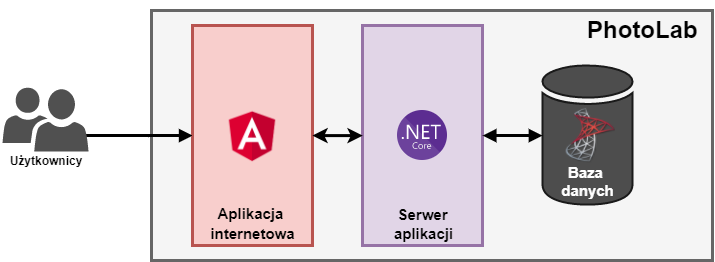
\includegraphics[width=1\linewidth]{graphics/chapter-4/general-application-architecture.png}
	\caption{Ogólny diagram architektury aplikacji \textit{PhotoLab}}
	\label{fig:general-application-architecture}
\end{figure}
\noindent Precyzując strukturę zademonstrowaną na rysunku \ref{fig:general-application-architecture}, należy poruszyć temat sposobu komunikacji między warstwami aplikacji i rodzajami użytkowników, którzy się z nią łączą.\\
	\\
	Temat użytkowników i ich dostępów zostanie poruszony szczegółowo w kolejnej sekcji. Na tym etapie wystarczy jedynie zaznaczyć, iż w systemie rozróżniane są trzy poziomy użytkowników: niezalogowany, zalogowany oraz administrator.\\
	\\
	Klient komunikuje się z aplikacją za pomocą licznych formularzy, przełączników i przycisków, natomiast serwis prezentuje żądane informacje w formie tekstowej, tabelarycznej oraz graficznie jako obrazy i wykresy.\\
	Przepływ danych pomiędzy warstwą kliencką, a serwerem aplikacji odbywa się poprzez zapytania (\textit{ang. request}) i odpowiedzi (\textit{ang. response}) \textit{HTTP} w postaci \textit{JSON}, czyli lekkiego formatu tekstowego bazującego na podzbiorze języka \textit{Javascript}.\\
	Wymiana danych serwera i bazy danych realizowana jest za pomocą tzw. \textit{ObjectModeli}, które są natywnym formatem obsługi wymiany informacji w  wykorzystywanym do tego narzędziu \textit{Entity Framework}. Uwzględniając dodatkowe informacje, można zmodyfikować poprzedni diagram do postaci przedstawionej na rysunku \ref{fig:application-architecture-without-payu}.
	
	
	
	
	\begin{figure}[ht]
	\centering
	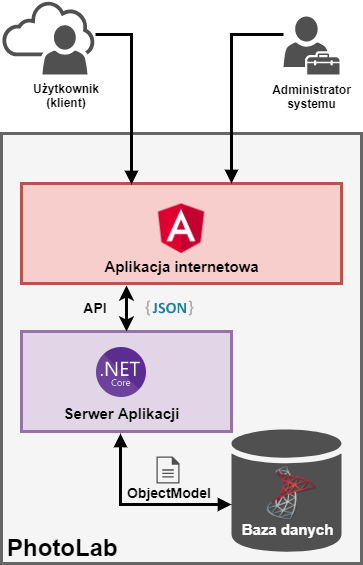
\includegraphics[width=0.5\linewidth]{graphics/chapter-4/application-architecture.png}
	\caption{Szczegółowy diagram architektury aplikacji \textit{PhotoLab}}
	\label{fig:application-architecture-without-payu}
\end{figure}
	
	
\noindent Głównym elementem, wokół którego operuje zasadnicza część aplikacji są \textbf{zlecenia}. To one umożliwiają złożenie zamówienia na wykonanie usługi, by następnie pracownik laboratorium na ich podstawie mógł wywołać odbitki oraz poinformować klienta o gotowym, oczekującym efekcie końcowym całego procesu. \\
	Każdemu etapowi zlecenia został przypisany odpowiedni stan, który jednoznacznie informuje zarówno klienta jak i pracownika zakładu o koniecznych do podjęcia krokach mających na celu zakończenie procesu sukcesem. Wszystkimi stanami zlecenia zarządza administrator systemu lub sam system czyni to automatycznie. Na poniższym diagramie został przedstawiony cykl życia zlecenia wraz z zaznaczonymi obszarami odpowiedzialności poszczególnych grup osób za zlecenie w danym stanie.
	
	\begin{figure}[ht]
    	\centering
    	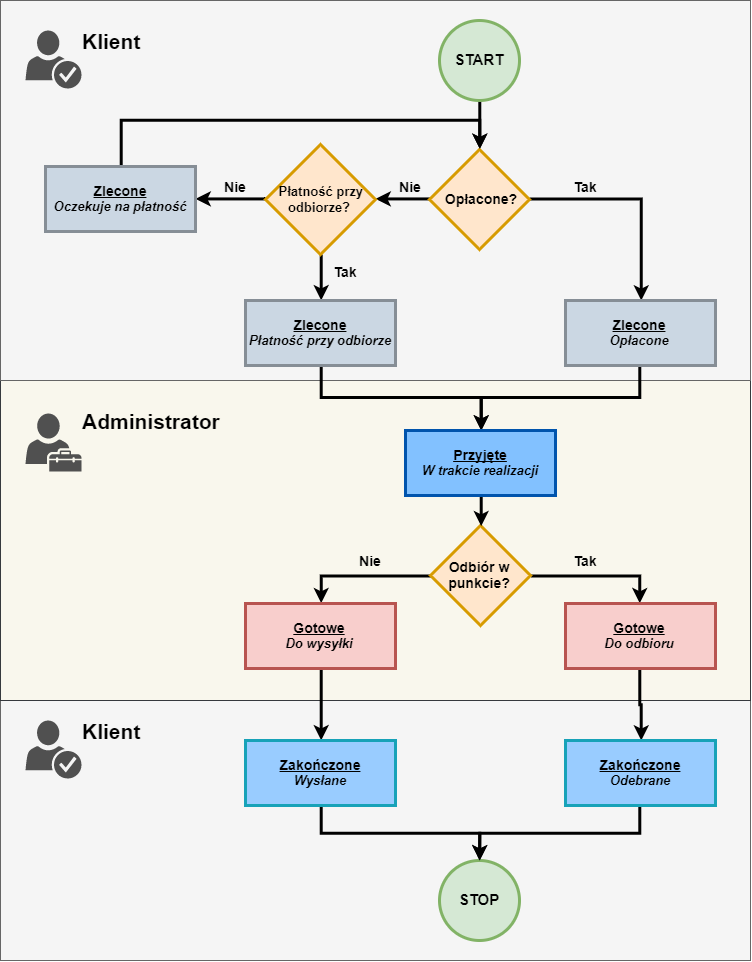
\includegraphics[width=0.9\linewidth]{graphics/chapter-4/order-states.png}
    	\caption{Cykl życia zlecenia}
    	\label{fig:order-states}
    \end{figure}
	
	\section{Dostęp i bezpieczeństwo}
	
\quad Serwis zapewnia zróżnicowany poziom dostępu na poziomie zarówno aplikacji internetowej, jak i serwera. Wyróżnione zostały \textbf{3 poziomy dostępu}:
	\begin{itemize}
	    \item \textbf{Użytkownik niezalogowany} - ma dostęp jedynie do podstawowych zasobów strony (głównie stron statycznych). Nie ma możliwości składania zleceń oraz dostępu do panelu administratora.
	    \item \textbf{Użytkownik zalogowany} - ma możliwość korzystania ze wszystkich użyteczności serwisu z modułu laboratorium. Brak możliwości zalogowania i użytkowania panelu administracyjnego.
	    \item \textbf{Administrator} - pełny dostęp do wszystkich możliwości serwisu.
	\end{itemize}
	
\noindent Po stronie \textit{Angular'a} ograniczenie dostępu odbywa się na poziomie \textit{routingu}, czyli wyznaczania ścieżki do podstron aplikacji. Służy do tego interfejs \textit{CanActivate} z paczki \textit{@angular/router}, który implementuje klasa ,,strażnika''.
	
\begin{listing}[ht]
    \jscode{listings/can-activate-interface.ts}
    \caption{Implementacja metody interfejsu \textit{CanActivate}}
    \label{listing:can-activate-interface}
\end{listing}

\noindent Tak stworzona klasa wstrzykiwana jest jako zależność do klasy odpowiedzialnej za sterowanie ruchem na stronie (\textit{router}), gdzie odpowiada za przydzielanie dostępu do odpowiedniej ścieżki adresu WWW.

\begin{listing}[ht]
    \jscode{listings/injection-auth-guard.ts}
    \caption{Wstrzyknięcie zależności \textit{AuthGuard} do klasy \textit{routing'u}}
    \label{listing:injection-auth-guard}
\end{listing}

\noindent Jak widać na powyższych listingach, w celu weryfikacji dostępu do danej sekcji strony sprawdzany jest status użytkownika (np. czy jest administratorem, lub czy jest zalogowany). Aby jednak aplikacja kliencka miała wiedzę dotyczącą przydzielonego poziomu dostępu, konieczna jest komunikacja z serwerem. Odbywa się to w momencie logowania do systemu - użytkownik wysyła dane logowania, system weryfikuje ich poprawność i zwraca odpowiedni \textit{Token JWT} wraz z informacjami o przydzielonych uprawnieniach.

\begin{listing}[ht]
    \cscode{listings/login-server.cs}
    \caption{Obsługa logowania użytkownika po stronie serwera}
    \label{listing:login-server}
\end{listing}

\noindent Tak otrzymaną odpowiedź należy jeszcze przetworzyć po stronie klienta. Służy do tego metoda \textit{login}, jednego ze stworzonych serwisów aplikacji (\textit{UserService}). W pierwszej kolejności wysyła ona zapytanie do serwera, które zostaje obsłużone przez metodę zaprezentowaną w~listingu powyżej. Następnie oczekuje na odpowiedź. Gdy takowa przyjdzie, należy ją obsłużyć. W przypadku aplikacji \textit{PhotoLab} jest to zapisanie \textit{tokena JWT} oraz identyfikatora użytkownika w lokalnej pamięci, ustawienie statusu jako \textit{,,zalogowany''} i ostatecznie zweryfikowanie, czy użytkownik posiada prawa administratora. 
\newpage
    
\begin{listing}[ht]
    \jscode{listings/login-client.ts}
    \caption{Obsługa logowania użytkownika po stronie klienta}
    \label{listing:login-client}
\end{listing}

\noindent Szczegółowe wyjaśnienie sposobu weryfikacji użytkownika za pomocą \textit{ASP.NET Identity} oraz standardu \textit{JWT Token} zostało zaprezentowane w rozdziale dotyczącym technologii warstwy logiki biznesowej (\textit{Rozdział 3.3.2}).\\
    Serwer aplikacji również posiada własny system weryfikacji dostępu użytkownika. Jest on zaimplementowany w postaci modułu \textit{ASP.NET Identity}, gdzie za poziom dostępu odpowiadają przydzielone użytkownikowi  prawa (\textit{ang. claims}). W momencie przekierowywania zapytania klienta do odpowiedniego kontrolera lub metody weryfikowane są prawa użytkownika (dostęp może być sprawdzany na jednym z dwóch lub na obu). Jeżeli zgłaszający zapytanie użytkownik posiada odpowiednie prawa, zapytanie jest realizowane. Jeżeli nie - zwracany jest błąd serwera w postaci kodu z numerem \textit{401} (\textit{Unauthorized}).
    
	\section{Serwer aplikacji i baza danych}
	
	\quad W sekcji tej zostanie omówiona architektura serwera aplikacji. Wyjaśnione zostaną kluczowe elementy tej warstwy wraz z przykładami w postaci listingu kodu. Poruszony zostanie również bardzo ważny temat bazy danych obsługującej cały serwis. Przedstawiona zostanie jej struktura, a także sposób komunikacji z serwisem.
	
\subsection{Struktura Web API}
\quad \textit{Web API} to bardzo ogólne pojęcie interfejsu korzystającego z protokołu \textit{HTTP} oraz formatu \textit{JSON} lub \textit{XML}. Pozwala na komunikowanie się użytkowników witryny z systemem aplikacji (serwerem) umieszczonym w dowolnej lokalizacji. \\
W przypadku aplikacji \textit{PhotoLab} została wdrożona implementacja  w postaci projektu \textit{ASP.NET Core Web API}. Ogólna struktura tego projektu przedstawiona została na rysunku \ref{fig:server-structure}.\\
Nie zagłębiając się w szczegółową budowę i strukturę projektu wygenerowanego przez oprogramowanie \textit{Visual Studio}, należy dostrzec jednak kilka kluczowych elementów serwera.

\begin{wrapfigure}[19]{l}{0.35\textwidth}
    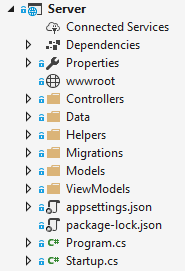
\includegraphics[width=1\linewidth]{graphics/chapter-4/server-structure.png}
    \caption{Struktura plików serwera aplikacji}
    \label{fig:server-structure}
\end{wrapfigure}

Najważniejsze z nich to foldery:
\begin{itemize}
    \item \textit{\textbf{Controllers}} - zbiór klas kontrolerów odpowiedzialnych za poszczególne działania, np. autentykację, użytkownika, obsługę zleceń czy statystyk serwisu. Kontroler jest klasą, która przechwytuje skierowane do niego zapytania \textit{HTTP}, przekazuje je do swojej odpowiedniej metody, która przetwarza informacje zgodnie z zaimplementowaną logiką, by następnie zwrócić je w postaci odpowiedzi \textit{HTTP}.
    \item \textit{\textbf{Data}} - zawiera klasę służącą do nawiązania połączenia z bazą danych.
    \item \textbf{\textit{Models}} - sekcja zawierają wszystkie modele obiektów, czyli reprezentantów informacji. Są one zbudowane jako klasy języka \textit{C\#}, zwane jako \textit{Plain Old C\# Object} (\textit{POCO}). Modele te, przekonwertowane przez \textit{Entity Framework} tworzą strukturę tabel bazy danych.
    \item \textbf{\textit{ViewModels}} - pakiet klas obiektów, nazywanych również \textit{DTO} (\textit{ang. Data Transfer Object}) służących do komunikacji serwera z aplikacją kliencką.
\end{itemize}

\noindent \textit{Web API} nie ma ustalonej i sztywno połączonej z nim aplikacji klienckiej. Dowolny serwis może nawiązać komunikację wykorzystując jedynie odpowiednie zapytania \textit{HTTP} skierowane pod ustalony adres. Z serwerem aplikacji \textit{PhotoLab} może łączyć się nie tylko specjalnie utworzony serwis oparty o \textit{Angular'a}, ale dowolny inny, np. nakierowany na działanie na urządzeniach mobilnych lub w przypadku testowania poprawności serwera (jak miało to miejsce w~czasie implementacji) - specjalnie przeznaczony do tego typu zabiegów program \textit{Postman}. 



\subsection{Baza danych}
\quad Ostatnią warstwą architektury trójwarstwowej jest baza danych. Serwis \textit{PhotoLab} to nie tylko wykonywane akcje, to również dane, na których operuje. Bez nich funkcjonowanie systemu byłoby niemożliwe. Większość działań podejmowanych na stronie odwołuje się do informacji przetrzymywanych właśnie w bazie danych. Znajdują się tam dane o~użytkownikach i~ich dostępach, złożonych zamówieniach, czy ustawieniach biznesowych (ceny, rodzaje papieru, możliwości wysyłki, płatności).\\
\\
Dzięki zastosowaniu narzędzia \textit{Entity Framework} i podejścia \textit{\textbf{Code First}} nie było konieczne tworzenie schematu bazy danych wprost \cite{entity-programming}. Podejście to definiuje, iż pierwszym etapem budowy bazy danych jest stworzenie typów w języku \textit{C\#}, które odpowiadają modelowi danych. Następnie w połączeniu z odpowiednimi adnotacjami umożliwiają one automatyczne wygenerowanie schematu bazy. Przykład jednego z najprostszych modeli całego systemu został przedstawiony na listingu poniżej:
\newpage

\begin{listing}[ht]
    \cscode{listings/model-server.cs}
    \caption{Model służący do budowy bazy danych}
    \label{listing:model-server}
\end{listing}

\noindent W ten sposób zbudowana klasa jest doskonałym reprezentantem tabeli, która zostanie na jej podstawie wygenerowana. Najważniejszym elementem tabeli jest kolumna zawierająca niepowtarzalny numer identyfikacyjny każdego rekordu. Jeżeli zostanie zachowana odpowiednia konwencja nazewnicza (tak, jak na powyższym przykładzie), nie jest nawet konieczne dodawanie adnotacji, informujących, iż dane pole ma służyć jako unikalny numer \textit{id}. Kolejne elementy listingu to pola typu \textit{string}, odpowiedzialne za generowanie kolumn, mających w tym konkretnym przypadku za zadanie przetrzymywanie informacji o adresie dostawy. Linie 9-11 to dwie \textit{propercje} i jedna adnotacja, które tak naprawdę odpowiedzialne są za wygenerowanie tylko jednej kolumny. Będzie ona zawierać klucz obcy do tabeli użytkowników, o czym informuje adnotacja \textit{ForeignKey}. Linia 11 służy tak naprawdę jedynie do tego, aby w~momencie, gdy zostaną pobrane dane o dostawie, można było również pobrać zależne od tych informacji dane o użytkowniku, np. za pomocą metody \textit{lazy loading} i metody \textit{Include}. W ten sposób o~wiele prościej jest operować na modelach pobranych z bazy danych.\\
\\Warto również pamiętać, iż w ten sposób stworzona klasa modelu nie jest jeszcze w pełni gotowa do zmapowania jej na tabelę bazy danych. Należy przedtem poinformować narzędzie, iż tak stwrzono model ma ono przetworzyć. Odbywa się to w metodzie \textit{PhotoLabContext} implementującej interfejs \textit{IdentityDbContext} poprzez komendę (np. dla powyższego modelu):

\begin{listing}[ht]
    \cscode{listings/adding-model-server.cs}
    \caption{Uwzględnienie modelu w budowaniu bazy danych}
    \label{listing:adding-model-server}
\end{listing}

\noindent Komenda ta informuje \textit{Entity Framework}, że ma on zmapować model \textit{DeliveryData} na tabelę o~nazwie \textit{DeliveryDatas}.\\
\\
W ten sposób wygenerowana baza danych systemu \textit{PhotoLab} składa się z 21 tabel. Relacje między poszczególnymi tabelami to zarówno jeden do jednego, jeden do wielu i wiele do wielu. W całym systemie można znaleźć również tabelę nie będącą w żadnej relacji. Odpowiada ona za przechowywanie statystyk wykonanych zdjęć legitymacyjnych w zakładzie, które nie są w żaden sposób uwzględnione w systemie jako jedna z usług, a dane na ich temat są przetrzymywane w aplikacji jedynie w celach statystyki biznesowej. \\
\\
\noindent Przed omówieniem całej struktury bazy danych warto zapoznać się z jej diagramem graficznym, który przedstawiony został na rysunku \ref{fig:database-scheme}.

\begin{figure}[ht]
    \centering
    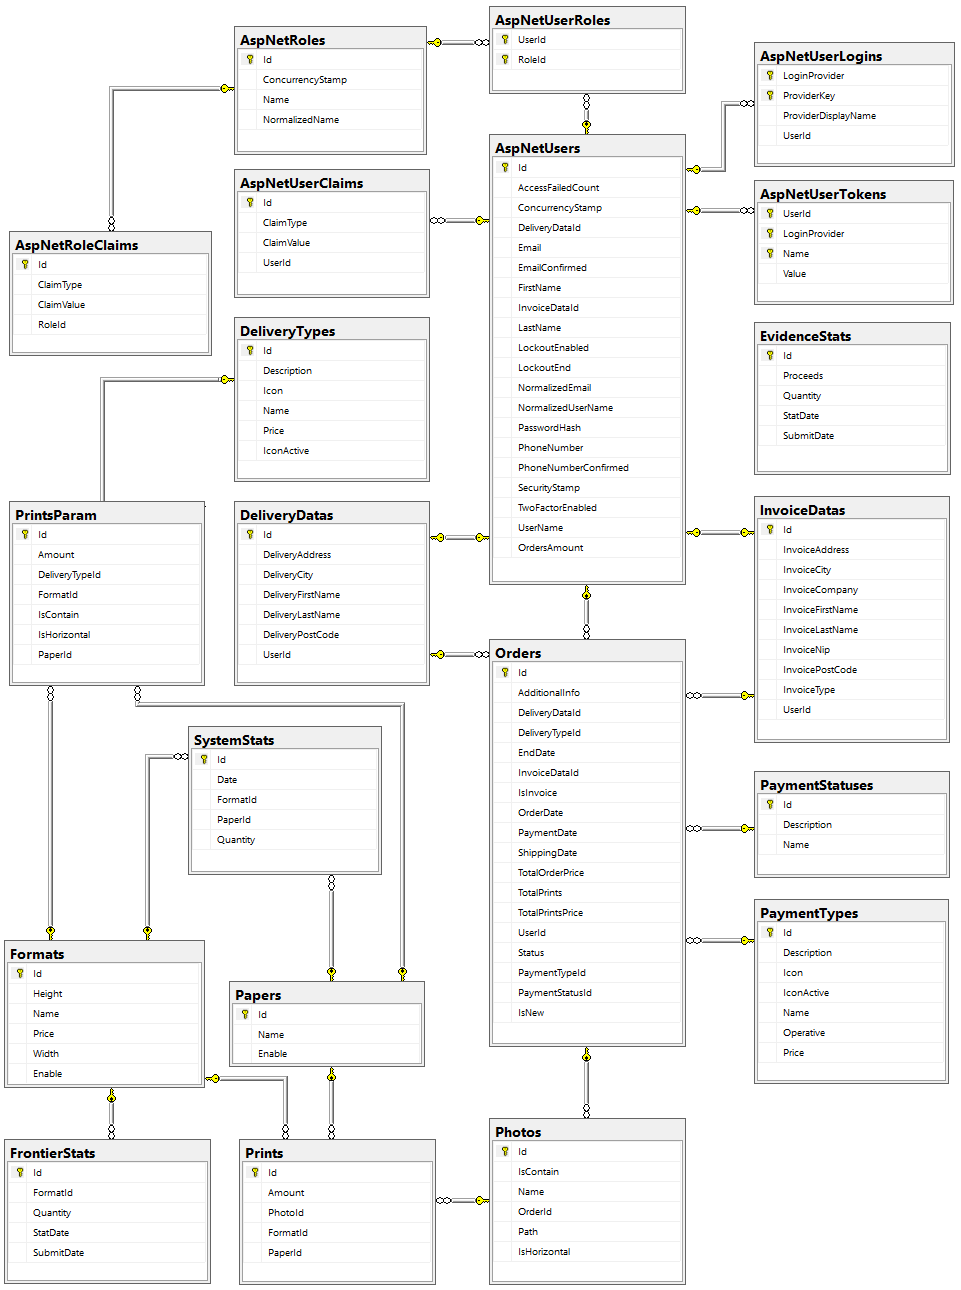
\includegraphics[width=1\linewidth]{graphics/chapter-4/database-scheme.png}
    \caption{Diagram architektury bazy danych}
    \label{fig:database-scheme}
\end{figure}



\noindent Siedem spośród przedstawionych na diagramie tabel (znajdujących się w górnej części rysunku) zawiera przedrostek \textit{AspNet}. Są to tabele wygenerowane automatycznie przez bibliotekę \textit{ASP.NET Identity} odpowiedzialną za system rejestracji i przydzielania ról użytkownikom. Tabela \textit{AspNetUsers} jako jedyna z nich posiada dodatkowe pola, które zostały dodane specjalnie na potrzeby aplikacji \textit{PhotoLab}. Wszystkie pozostałe przedstawione na diagramie tabele zostały wygenerowane poprzez przygotowanie ich odpowiednich modeli i wykorzystanie narzędzia do zmapowania ich na \textit{SQL-owe} polecenia odpowiedzialne za wygenerowanie tabel. Rdzeniem całego systemu są dwie nie tylko ,,największe'' (zawierające największą ilość atrybutów) ale i najważniejsze tabele: użytkownicy i zlecenia. Poza modułem statystyk, który funkcjonuje nieco z boku głównej funkcjonalności systemu (zamówień), wszystkie inne tabele powiązane są bezpośrednio lub pośrednio z tymi dwoma tabelami. Wartymi objaśnień wydają się powiązania z tabelą \textit{Orders}. Jak widać, każde zlecenie może mieć tylko i wyłącznie jednego właściciela (\textit{AspNetUsers}), który to z kolei może w swojej historii być twórcą wielu zleceń, a do konta mieć przypisany jeden adres dostawy. Spoglądając na powiązania z tabelą \textit{Orders} po prawej stronie diagramu widać, iż każde zlecenie zawiera takie informacje jak: rodzaj i status płatności, a~także dane do faktury i (powiązanie z lewej strony diagramu) dane do ewentualnej wysyłki (jeśli użytkownik zaznaczy takową opcję). Bardzo ważna częścią każdego zamówienia są informacje odnośnie przesłanych przez użytkownika zdjęć i parametrach ich wydruku. Informacje te zawarte są w tabeli \textit{Photos}, która występuje w relacji jeden do wielu w stosunku do tabeli \textit{Orders}. Każde zamówienie posiada listę zdjęć wgranych przez klienta do systemu. Każde zdjęcie zawiera ogólne informacje, np. o ścieżce do lokalizacji na serwerze, jego nazwie czy sposobie dopasowania w czasie wydruku, a także co najważniejsze - odwołanie do kolejnej tabeli posiadającej informacje o szczegółach dotyczących rozmiaru odbitki, papieru na którym ma zostać nadrukowana i ilości sztuk.\\
\\
Modułem niezwykle ważnym z biznesowego punktu widzenia, jednak mniej, niż moduł zleceń, związanym z całą strukturą bazy danych jest moduł statystyk laboratorium. W jego skład wchodzą trzy tabele, czyli dokładnie tyle, ile typów statystyk jest prowadzonych w ramach serwisu. Są to kolejno:
\begin{itemize}
    \item \textit{SystemStats} - generowany automatycznie, codzienny raport o wszystkich zleceniach zrealizowanych z poziomu serwisu,
    \item \textit{FrontierStats} - informacje wprowadzane ręcznie przez właściciela zakładu, comiesięczne informacje o ilości wydrukowanych zdjęć na maszynie \textit{Frontier},
    \item \textit{EvidenceStats} - również wprowadzane ręcznie, codzienne statystyki o ilości wykonanych zdjęć legitymacyjnych.
\end{itemize}


\noindent Tabele \textit{SystemStats} i \textit{FrontierStats} ściśle powiązane są z tabelami \textit{Formats} i \textit{Papers} (\textit{FrontierStats} tylko z \textit{Formats}), gdzie wyświetlają odpowiednie dane statystyczne na podstawie typów formatów i papierów. Bardzo ważnym elementem implementacji bazy danych było zapewnienie spójności danych. Należało przewidzieć zjawisko, gdzie mógłbym zostać usunięty jeden z~wcześniej dostępnych formatów lub papierów. Wówczas wszystkie powiązania związane z zamówieniem i statystykami do tych parametrów uległyby zniszczeniu, a system zawierałby ubytki w informacjach. Aby uniknąć tego zjawiska został zaimplementowany mechanizm uniemożliwiający usunięcie encji, dla których istnieje już jakiekolwiek powiązanie w systemie. Możliwym rozwiązaniem jest wówczas dezaktywacja takiego wariantu, tak aby nie był on już brany pod uwagę w dalszej pracy systemu, natomiast pozwolił zachować pełną historię wykonywanych operacji.
\newpage

\vspace*{0.01\baselineskip}

\subsection{Przetwarzanie zapytań}
\quad Głównym zadaniem serwera, którego ogólny zarys został nakreślony już we wcześniejszej części, jest przetwarzanie zapytań. W sekcji tej zostanie zaprezentowany konkretny przykład przetwarzania dwóch bardzo ważnych zadań: tworzenia zamówienia oraz wyświetlania listy wszystkich zleceń przez administratora systemu.\\
\\
\textit{Request} w postaci:

\vspace{2mm}

    \centerline{\texttt{\hl{ adres-serwera:port/api/order/submitorder }}}

\vspace{2mm}

\noindent wraz z przesyłanymi danymi oraz załączonymi w postaci nagłówków informacjami o~sposobie kodowania zapytania oraz \textit{tokenem JWT} umożliwiającym weryfikację praw dostępu użytkownika, wysyłany jest do serwera. Tam, z pomocą zaimplementowanego \textit{routing} przekierowywany jest najpierw do odpowiedniej klasy, a następnie metody - uwzględniając przy tym prawa dostępu użytkownika.\\
Tym sposobem serwer aplikacji otrzymuje od użytkownika wszystkie konieczne do założenia nowego zlecenia dane. Ponieważ użytkownik ma szeroki zakres możliwości przy konfiguracji swojego zlecenia, nie można tak otrzymanego zapytania natychmiast zapisać w bazie danych. Należy je najpierw odpowiednio przetworzyć. Dzieje się to w metodzie \textit{SubmitOrder}, klasy \textit{PhotoController}. 

\begin{listing}[ht]
    \cscode{listings/submit-order-server.cs}
    \caption{Obsługa zapytania stworzenia nowego zlecenia}
    \label{listing:submit-order-server}
\end{listing}

\noindent Parametr metody \textit{OrderVM} to otrzymane poprzez część \textit{body} zapytania HTTP dane z wypełnionego przez użytkownika formularza zlecania zamówienia. Tak otrzymane informacje w~postaci \textit{JSON} automatycznie konwertowane są na \textit{C\#-owy} \textit{ViewModel}. W przypadku powyższego zapytania ma on postać: 

\begin{listing}[ht]
    \cscode{listings/viewmodel-order-server.cs}
    \caption{\textit{ViewModel} zamówienia przesyłany do serwera aplikacji}
    \label{listing:viewmodel-order-server}
\end{listing}

\noindent Jest to zwykła klasa zawierająca listę prywatnych pól wraz z domyślnymi metodami \textit{get} i~\textit{set} do ich obsługi. Wracając do \textit{listingu \ref{listing:submit-order-server}} - tak określony model jest w linii 5 sprawdzany pod względem poprawnościowym. W przypadku niezgodności - zwracany jest błąd, a funkcja kończy działanie. Jeśli wszystko jest w porządku, przetwarzane są informacje dotyczące ewentualnej wysyłki i faktury za zamówienie. Ponieważ użytkownik ma możliwość w obu przypadkach podjęcia decyzji: czy wysyłka lub faktura jest konieczna - jeśli nie, weryfikacja ta jest pomijana, a do bazy danych zostaje zapisana bezpośrednia informacja otrzymana od klienta o braku danych na ten temat. Jeżeli użytkownik zdecyduje się na któryś z wariantów, ponownie podejmuje decyzję. Możliwe wybory to wykorzystanie danych przypisanych do jego konta lub podanie nowych informacji, przypisanych wyłącznie do tego zlecenia. Właśnie te informacje są interpretowane w liniach od 7 do 14 (ze względu na obszerność kodu, analogiczne operacje zostały pominięte). Linia numer 15 to zmapowanie, za pomocą dodatkowej biblioteki \textit{\textbf{AutoMapper}}, odpowiednio przetworzonych danych do pól modelu \textit{Order}. Kolejne linie kodu to dodanie tak utworzonego zlecenia oraz jego zależności w~postaci informacji o~zdjęciach i~konkretnych odbitkach do kontekstu (\textit{\_context}). Gdy proces ten zostanie ukończony, wystarczy zapisać zmiany w bazie danych i zwrócić odpowiedni komunikat rezultatu zapytania.\\
\\
Drugi przykład obsługi żądań przez serwer to zapytanie typu \textit{GET} - typ zapytania, które nie wysyła żadnych informacji w swojej treści, a jedynie prosi serwer o zwrócenie konkretnych danych. Omawiane zapytanie wysyłane jest pod adres:

\vspace{2mm}

    \centerline{\texttt{\hl{ adres-serwera:port/api/order/getorders }}}

\vspace{2mm}

\noindent trafiając w ten sposób do metody wskazanej w listingu poniżej.

\begin{listing}[ht]
    \cscode{listings/getorders-server.cs}
    \caption{Obsługa zapytania zwrócenia wszystkich zleceń}
    \label{listing:getorders-server}
\end{listing}

\noindent Sposób działania tej metody jest bardzo prosty. W pierwszej kolejności pobiera ona z bazy danych wszystkie znajdujące się w niej zlecenia i zapisuje w postaci listy. Poprzez dyrektywę \textit{Include} do pobranych zleceń za pomocą tzw. ładowania danych \textit{lazy loading} dołączone są informacje o użytkowniku zlecającym zamówienie. Następnie tworzona jest lista nowych, pustych \textit{ViewModeli}, które wypełniane są danymi otrzymanymi z bazy danych. Zabieg ten ma na celu ograniczenie ilości informacji,  które mają zostać przekazane aplikacji klienckiej, a zostały pobrane z bazy danych. Po pierwsze ma to wskazania wydajnościowe, po drugie bezpieczeństwa, a po trzecie ułatwia to późniejsze obsługiwanie tak uproszczonych i nie przeładowanych zawartością zapytań. Ostatnim etapem jest zwrócenie utworzonej listy i odpowiedzi z kodem typu \textit{200}.


\section{Aplikacja internetowa}
\quad Pierwsza warstwa modelu trójwarstwowego to aplikacja ukierunkowana na interakcję z użytkownikiem. Zaimplementowana jako projekt oparty o \textit{framework} \textit{Angular 4.4.6}, została podzielona na 3 podstawowe moduły, które zostaną szczegółowo nakreślone w tym rozdziale.
\newpage

\vspace*{0.01\baselineskip}

\subsection{Architektura aplikacji SPA}

        \begin{wrapfigure}[20]{l}{0.35\textwidth}
        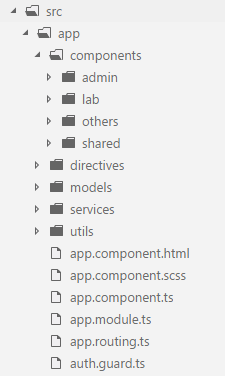
\includegraphics[width=1\linewidth]{graphics/chapter-4/client-structure.png}
        \caption{Struktura plików aplikacji klienckiej}
        \label{fig:client-structure}
        \end{wrapfigure}
            Zasadnicza struktura projektu zawarta jest w folderze \textit{src/app}. Zawiera takie elementy jak:
    \begin{itemize}

        \item Folder \textit{\textbf{components}} - zawierający komponenty czyli podstawowe składowe projektu dodatkowo podzielone na podfoldery rozdzielające poszczególne moduły aplikacji.
        \item Folder \textit{\textbf{directives}} - zbiór dodatkowych funkcjonalności, które dołączane są do \textit{drzewa DOM} dokumentu HTML w trakcie jego kompilacji.
        \item Folder \textit{\textbf{models}} - struktury odpowiedzialne za obiekty wykorzystywane w aplikacji oraz w komunikacji z serwerem.
        \item Folder \textit{\textbf{services}} - pakiet funkcji odpowiedzialnych za komunikację z serwerem i przetwarzanie rezultatów na poziomie abstrakcji danych.
        \item Pliki z serii \textit{\textbf{app}} - główne pliki \textit{Angular}, to od ich przetworzenia rozpoczyna swoje działanie cały projekt.
        \item Plik \textbf{\textit{AuthGuard}} - implementuje interfejs \textit{CanActivate}, definiując w ten sposób wymagania odpowiedzialne za dostęp do poszczególnych komponentów.
    \end{itemize}
Najważniejsza jest jednak logika podziału aplikacji na moduły i sekcje, które decydują o możliwościach jakie serwis udostępnia poszczególnym grupom użytkowników. Podział na moduły został oparty o bardzo prostą logikę poziomu dostępów oraz sposobu prezentacji witryny. Wyróżnione zostały \textbf{dwa moduły}: \textbf{administratora} oraz \textbf{laboratorium}.
\begin{figure}[ht]
	\centering
	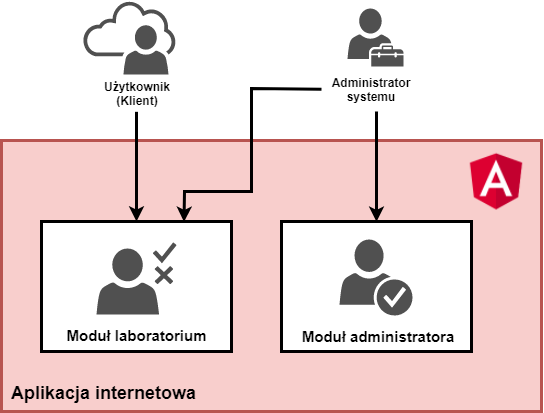
\includegraphics[width=0.75\linewidth]{graphics/chapter-4/client-architecture.png}
	\caption{Szczegółowy diagram architektury aplikacji klienckiej}
	\label{fig:client-architecture}
\end{figure}
Pierwszy z nich dostępny jest jak sama nazwa wskazuje jedynie dla osób posiadających status administratora strony. Przygotowany jest w formie panelu administracyjnego z bocznym panelem zarządzania w postaci \textit{sidebar'a}. \\Moduł laboratorium to cała dostępna dla użytkownika strona kliencka w skład której wchodzi zarówno wizytówka firmy jako strony statyczne aplikacji, jak i cały moduł zarządzania kontem użytkownika i zlecenia zamówień. Uwzględniony tam został również podział na użytkowników zalogowanych i niezalogowanych, jednak szczegółowe dotyczące dostępu do konkretnych sekcji zostaną omówione później.

\newpage
\subsubsection{Moduł Administratora}
\quad Dostęp do tej części serwisu umożliwiony jest jedynie dla zalogowanych (wyjątkiem jest strona logowania) użytkowników posiadających prawa administratora. Umożliwia on zarządzanie serwisem \textit{PhotoLab} poprzez funkcjonalności podzielone na odpowiednie podstrony tematyczne:
 \begin{itemize}
     \item \textbf{Kokpit} - składający się jedynie na podsumowanie najważniejszych informacji i statystyk dotyczących serwisu \textit{PhotoLab}.
     \item \textbf{Statystyki} - prezentacja tabelaryczna oraz w postaci wykresów wraz z możliwością dodawania i edycji danych dotyczących 3 zakresów statystyk:
        \begin{itemize}
            \item zleceń złożonych przez portal,
            \item wykonanej przez laboratorium liczby odbitek poszczególnych formatów w miesiącu,
            \item liczby wykonanych w ciągu dnia roboczego zdjęć legitymacyjnych.
        \end{itemize}
    \item \textbf{Zamówienia} - lista wszystkich zleceń z możliwością podglądu szczegółów oraz edycji niektórych parametrów zamówienia.
    \item \textbf{Użytkownicy} - podstrona prezentująca wszystkich zarejestrowanych użytkowników serwisu wraz z możliwością ich pełnej edycji.
    \item \textbf{Moje Konto} - zarządzanie ustawieniami konta obecnie zalogowanego użytkownika.
    \item \textbf{Preferencje} - sterowanie parametrami określającymi sposób działania serwisu, a także oferowanymi usługami i ich formą.
 \end{itemize}
Cały moduł oparty jest o główny komponent o nazwie \textit{layout}. Zawiera on ogólną strukturę całego szablonu panelu administracyjnego, wewnątrz którego wywoływane są inne moduły (w~oparciu o \textit{routing} aplikacji).

\begin{listing}[ht]
    \htmlcode{listings/admin-layout.html}
    \caption{Layout moduły administratora aplikacji klienckiej}
    \label{listing:admin-layout}
\end{listing}

\noindent W linii 4 i 5 importowane są statyczne komponenty nagłówka i bocznego panelu zawierającego logo oraz menu aplikacji. W linii 9 znajduje się dyrektywa odpowiedzialna za generowanie odpowiednich komponentów zgodnie ze wskazaniami \textit{trasowania}. Każdy komponent aplikacji \textit{Angular} składa się z trzech plików:
\begin{itemize}
    \item \textbf{\textit{.html}} - odpowiedzialny za generowanie struktury strony WWW,
    \item \textbf{\textit{.scss}} - plik prekompilatora \textit{Sass}, który w trakcie budowania aplikacji jest automatycznie kompilowany do kodu \textit{css} odpowiedzialnego za prezentację witryny,
    \item \textbf{\textit{.ts}} - zasadnicza część każdego komponentu - plik języka \textit{typescript} - który ostatecznie kompilowany jest do kodu języka \textit{javascript}. Jest to klasa wzbogacona o odpowiednie metadane, które pozwalają identyfikować ją jako komponent. Bazowa część komponentu to: selektor reprezentujący komponent, wskaźnik na plik szablonu i stylów oraz dodatkowe funkcje wywoływane pod wpływem zmiany stanu komponentów, jego rodzica, krewnego, potomków lub z poziomu \textit{drzewa DOM}.
\end{itemize}

\begin{figure}[ht]
	\centering
	
\includegraphics[width=0.75\linewidth]{graphics/chapter-4/order-component.png}
	\caption{Budowa komponentu \textit{Angular 4}}
	\label{fig:order-component}
\end{figure}
\noindent Struktury pliku \textit{.ts} jednego z najprostszych komponentów zaimplementowanych w serwisie, odpowiedzialnego za wyświetlanie listy zleceń w panelu administratora została przedstawiona na kolejnym listingu:
\newpage

\begin{listing}[ht]
    \jscode{listings/component-client.ts}
    \caption{Komponent modułu administratora serwisu \textit{PhotoLab}}
    \label{listing:component-client}
\end{listing}

\noindent W celu analizy powyższego kodu należy poruszyć kilka zagadnień:
\begin{enumerate}
    \item Linie 1-4 to import potrzebnych do obsługi komponentu danych z innych paczek, serwisów i modeli.
    \item Linie 6-10 to wspomniany wyżej dekorator zawierający alias komponentu oraz ścieżki do załączenia plików \textit{html} i \textit{css}.
    \item Od linii numer 11 zaczyna się zasadnicza część klasy komponentu. Występuje tam jego nazwa oraz informacja o implementacji dodatkowego interfejsu składającego się z jednej metody \textit{OnInit}.
    \item W konstruktorze klasy wstrzykiwana jest zależność serwisu odpowiedzialnego za obsługę zamówień (dokładne omówienie serwisów zostanie przedstawione w kolejnej sekcji).
    \item Linie 14-16 to deklaracja pól klasy wraz z inicjalizacją obiektu \textit{OrderState}.
    \item Kolejne linie to trzy funkcje: Linia 21 to implementacja interfejsu \textit{OnInit} - metoda ta wywoływana jest tylko raz, w początkowej fazie życia komponentu, tuż po wykonaniu się kodu konstruktora i pierwszego wywołania niezaimplementowanego w tym przykładzie interfejsu \textit{OnChanges}. Funkcja ta wywołuje kolejną metodę odpowiedzialną za wywołanie funkcji pobierającej dane o zamówieniu z bazy danych, znajdującej się we wstrzykniętym serwisie.
    \item Metoda \textit{getStatusName()} wywoływana jest z poziomu struktury \textit{DOM} komponentu w momencie konieczności wyświetlenia nazwy statusu zlecenia, a nie wyłącznie jego numeru.
\end{enumerate}
\subsubsection{Moduł Laboratorium}

\quad Ta część serwisu dostępna jest zarówno dla osób zalogowanych jak i anonimowych użytkowników. Podstrony objęte restrykcją dostępu są niedostępne dla użytkownika z poziomu interfejsu wystawionego przez aplikację kliencką oraz dodatkowo objęte weryfikacją posiadanych przez użytkownika uprawnień i statusu (zalogowany / niezalogowany). Przykładowo uniemożliwia to dostęp do chronionej strony poprzez wprowadzenia znanego adresu \textit{URL} do paska adresu przeglądarki internetowej. Zakres stron objętych koniecznością zalogowania użytkownika przedstawia poniższy schemat.

\begin{figure}[ht]
	\centering
	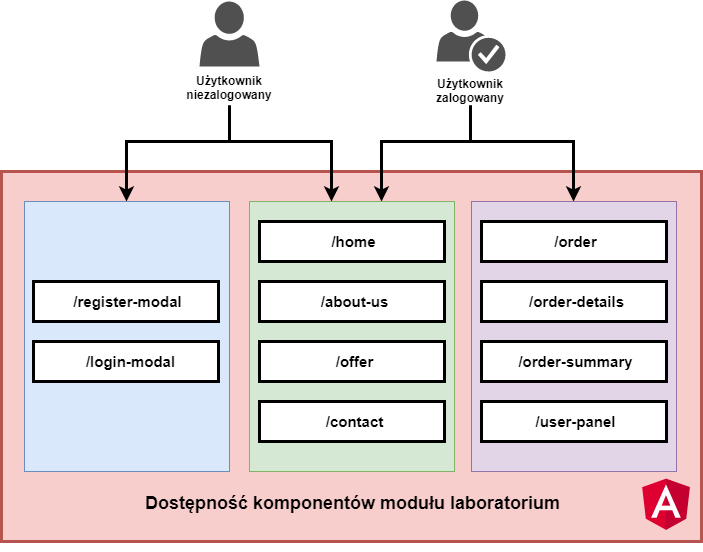
\includegraphics[width=0.8\linewidth]{graphics/chapter-4/lab-module-availability.png}
	\caption{Diagram Dostępności komponentów modułu laboratorium}
	\label{fig:lab-module-availabelity}
\end{figure}

\noindent Wszystkie strony znajdujące się na tle zielonym są to strony statyczne, tj. takie, które zawierają jedynie czysty kod \textit{html} i \textit{css}, bez dodatków w postaci dynamicznie ładowanych treści czy zachowań. Strony w niebieskim pudełku to 2 formularze służące kolejno do rejestracji nowego użytkownika oraz logowania użytkownika znajdującego się już w bazie systemu. Skonstruowane zostały w~formie tzw. \textit{okien modalnych } (\textit{modali}), czyli takich okien, które pojawiają się nad obecnie prezentowaną warstwą strony, wygaszając w ten sposób jej wszystkie funkcjonalności i powodując skupienie wzroku użytkownika (często poprzez przyciemnienie tła) na prezentowanych treściach - w tym wypadku na formularzach. \textit{Modal} znika w~momencie kliknięcia przez użytkownika jednego z proponowanych przycisków, np. \textit{anuluj} lub \textit{zapisz}/\textit{wyślij}, wykonując konkretną akcję i~powracając do widoku strony dostępnej przed pojawieniem się okna (lub przekierowując do akcji wybranej przez użytkownika).\\
\\
Również w tym module najważniejszą częścią są komponenty generujące konkretne strony lub ich fragmenty. Nie różnią się one jednak w żaden znaczący sposób od przykładowego komponentu zaprezentowanego w sekcji dotyczącej modułu administratora, dlatego też nie zostaną zaprezentowane ponownie. Pokazana natomiast zostanie budowa innych, równie ważnych elementów aplikacji \textit{Angular} - serwisów i modeli. \\
\\
Podobnie jak w aplikacji serwerowej opartej o język programowania \textit{C\#}, modele w aplikacji klienckiej służą po pierwsze do \textit{parsowania} ich do łatwo \textit{przenaszalnego} formatu~-~w~tym wypadku \textit{JSON} - by następnie mogły zostać wysłane w postaci zapytania HTTP jako dane do przetworzenia przez serwer. Drugim (nierozerwalnie powiązanym z pierwszym) zastosowaniem modeli jest przetrzymywanie informacji o danym typie danych oraz ich prezentacja i modyfikacja poprzez graficzny interfejs użytkownika w postaci strony \textit{html}. 
Przykładowa klasa modelu identycznego do tego zaprezentowanego w implementacji serwerowej została przedstawiona poniżej:

\begin{listing}[ht]
    \jscode{listings/model-client.ts}
    \caption{Model zlecenia w aplikacji klienckiej}
    \label{listing:model-client}
\end{listing}

\noindent Jedyną różnicą w prezentowanej strukturze (w porównaniu z implementacją serwerową) jest fakt zastosowania składni innego języka programowania (\textit{Typescript} vs. \textit{C\#}). Różnicą, jaką można zauważyć to definiowanie wszystkich pól automatycznie jako publiczne oraz umiejscowienie ich jako parametry konstruktora klasy. Jest to celowy zabieg umożliwiający w \textit{Typescript}  definiowanie elementów klasy automatycznie z określaniem ich parametrów dla domyślnego konstruktora bezparametrowego. W ten sposób można wyzbyć się nadmiernego tworzenia prawie identycznego kodu.\\
\\
\noindent W klienckiej aplikacji \textit{Photolab} serwisy pełnią cztery zasadnicze role:
\begin{itemize}
    \item jako jedyne struktury zawierają funkcje odpowiedzialne za komunikację z serwerem,
    \item zawierają metody, które są wykorzystywane przez co najmniej dwa komponenty jednak zazwyczaj są to metody, które wywoływane są w większości komponentów w tej samej formie. Ich implementacja w poszczególnych komponentach byłaby niepotrzebną redundancją kodu,
    \item przechowują obiekty, których okres występowania nie ogranicza się jedynie do jednego komponentu (np. obiekt \textit{order} - występuje w całym procesie zlecania zamówienia, tj. w~komponentach: \textit{order}, \textit{orderDetails} i \textit{orderSummary}),
    \item służą jako pośrednik w wymianie informacji pomiędzy komponentami, np. poprzez rozgłaszanie informacji do nasłuchujących komponentów.
\end{itemize}

\noindent Wszystkie powyżej wymienione funkcjonalności serwisów zostały zaprezentowane w~listingu \ref{listing:service-client} przedstawiającym fragmenty serwisu \textit{Order} służącego do obsługi procesu zlecania zamówienia w module laboratorium.

\begin{listing}[ht]
    \jscode{listings/service-client.ts}
    \caption{Serwis obsługi zlecania zamówień w module laboratorium}
    \label{listing:service-client}
\end{listing}

\noindent Linie 3-8 to pola dostępne do użytku wewnętrznego przez serwis lub do udostępnienia jednolitych danych wielu komponentom (np. pole \textit{order}). Metoda \textit{getFormatPrice(...)} to doskonały przykład bardzo prostej funkcji wykorzystywanej przez wiele komponentów w celu zwrócenia ceny formatu odbitki posiadając jedynie wiedzę o jej numerze identyfikacyjnym. Kolejna funkcja \textit{setOrderStatus(...)} jest egzemplarzem rodziny funkcji wysyłającej do serwera zapytanie \textit{HTTP}. W tym przypadku jest to zapytanie typu \textit{GET} proszące o zwrócenie liczby (oczekiwanie wartości typu \textit{Observable<number>}) zleceń ze statusem ,,nowe''. Gdy taka odpowiedź nadejdzie, należy ją zwrócić w postaci rezultatu wykonania funkcji lub w przypadku błędu przekierować go do funkcji wstrzykniętego do klasy serwisu \textit{ConfigService} odpowiedzialnego za obsługę błędów zapytań po stronie aplikacji. Ostatnia z głównych funkcjonalności serwisów została zaprezentowana na przykładzie w linii 24. Jest to funkcja odpowiedzialna za propagowanie wiadomości o zaistniałym zdarzeniu do innego, nasłuchującego na ten typ wiadomości kontrolera.
\newpage
\subsection{Warstwa prezentacji}
\quad Tworząc aplikację dostępną dla szerokiego grona użytkowników bardzo ważne jest zadbanie o~spójny, estetyczny wygląd oraz łatwą i intuicyjną strukturę serwisu, a także wyeksponowanie najważniejszych z biznesowego punktu widzenia elementów strony.\\
\\
Aby osiągnąć takowy efekt konieczne jest zbudowanie poprawnej oraz logicznej struktury \textit{drzewa DOM}, a także zapewnienie odpowiedniej formy prezentacji tych danych przy wykorzystaniu \textit{kaskadowych arkuszy stylów} (\textit{css}). W celu ułatwienia i stanowczego przyspieszenia prac w~projekcie został zaimplementowany \textit{framework CSS} - \textit{\textbf{Bootstrap}} w obecnie najnowszej wersji \textit{4.0.0} (będącej jeszcze wersją beta).\\
\\
Najważniejszymi elementami wykorzystanymi z tej biblioteki były przede wszystkim klasy opisujące strukturę dokumentu, tj. \textbf{\textit{FlexBox}} i \textbf{\textit{Bootstrap Grid}}. Ich implementacja była stosowana zamiennie lub w sposób mieszany w zależności od złożoności i konkretnych wymagań danej sekcji.\\
\\
Zamiast zwykłej składni \textit{CSS} (\textit{.css}) została użyta składnia preprocesora \textit{SASS} (\textit{.scss}) umożliwiającego bardziej zaawansowane operowanie na kaskadowych arkuszach stylów poprzez różnego rodzaju \textit{mixiny}, \textit{zmienne}, \textit{zagnieżdżenia}, itp. Przykład kilku wybranych fragmentów kodu implementujących najwięcej funkcjonalności udostępnianych przez preprocesor języka \textit{CSS} został przedstawiony poniżej:

\begin{listing}[ht]
    \sasscode{listings/sass-example.scss}
    \caption{Demonstracja możliwości preprocesora \textit{Sass}}
    \label{listing:sass-example}
\end{listing}

\noindent Powyższy kod wydaje się być na tyle prosty i intuicyjny, iż nie wymaga większych objaśnień. \textit{@mixin} to zestawy reguł zebranych pod jednym \textit{aliasem}, które bez zbędnych powtórzeń można wykonywać wielokrotnie w kodzie. Znakiem \textit{\$} rozpoczyna się nazwa zmiennej, do której np. można przypisać odpowiednią wartość koloru. Następnie w momencie potrzeby zmiany odcieniu wszystkich elementów \textit{ostylowanych} danym rodzajem koloru, nie jest konieczne dokonywanie zmian w wielu miejscach, wystarczy jedna zmiana, w definicji zmiennej. \\
\\
Aplikacja \textit{PhotoLab} to jednak nie tylko efekty generowane przez arkusze stylów. To również liczne grafiki, ikony i obrazy. Wszystkie wymienione (z wyjątkiem kilku elementów, które są własnością autora pracy) zostały zaczerpnięte z licznych stron internetowych. W~trakcie ich selekcji zostały uwzględnione ustanowione dla nich prawa autorskie. Większość wykorzystanych fotografii pochodzi z serwisu \textit{Pexels.com}, który udostępnia wysokiej jakości fotografie w~większości na licencji \textit{CC0} - oznaczającej ,,Brak zastrzeżonych praw autorskich'' (\textit{ang. no copyright reserved}). Natomiast jeżeli chodzi o wykorzystane ikony, to ich jedynym źródłem jest portal \textit{FontAwesome.io} oferujący dodatkową bibliotekę udostępniającą szeroki zakres ikon w postaci wektorów, które można dostosowywać do własnych potrzeb poprzez zmianę np. koloru czy rozmiaru. Ikony te udostępnianie są na licencji \textit{SIL Open Font License}, oznaczającą pełną dowolność w ich wykorzystaniu.
\newpage

\vspace*{0.01\baselineskip}

\section{Środowisko produkcyjne}
\quad Aplikacja w trakcie procesu jej powstawania była budowana, uruchamiana i testowana w oparciu o \textit{\textbf{środowisko deweloperskie}}. Różni się ono od \textit{\textbf{środowiska produkcyjnego}} w kilku aspektach. Ogólnie mówiąc otoczenie programistyczne zawiera więcej dodatkowych informacji mających na celu możliwość \textit{debugowania} i sprawdzenia tworzonego kodu. Pliki nie są w pełni skompresowane, a np. ścieżki odnoszą się często do innych, również tymczasowych (na czas implementacji) lokalizacji. Dodatkowo należy zaznaczyć, iż cały proces budowania i uruchamiania aplikacji odbywa się (w przypadku \textit{PhotoLab}) lokalnie na komputerze programisty. Tak wygenerowany projekt nie może być po prostu przeniesiony 1:1 na zewnętrzny hosting. Należy go odpowiednio przygotować i osadzić na odpowiednim do tego serwerze, a następnie uruchomić. Konieczne do zakończenia tego procesu sukcesem kroki zostały przedstawione w tej części rozdziału. Na koniec została umieszczona również skrócona instrukcja użytkowania aplikacji prezentująca jego najważniejsze elementy i funkcjonalności.

\subsection{Proces instalacji}
\quad W tej sekcji zostanie zaprezentowana ogólna instrukcja postępowania mającego na celu wygenerowanie projektu w wersji produkcyjnej oraz jego późniejsze wdrożenie (\textit{ang. deploy}) na zewnętrznym serwerze pełniącym rolę hostingu aplikacji.\\
\\
Zaprezentowany sposób nie jest z pewnością najbardziej optymalny i służący do masowego i ciągłego aktualizowania wersji produkcyjnej oprogramowania. Rozwiązanie takie można zautomatyzować, np. w taki sposób aby wszelkie zmiany naniesione w projekcie i~zapisane na zdalnym repozytorium były automatycznie wdrażane na serwer produkcyjny. Na potrzeby aplikacji \textit{PhotoLab} proces przygotowywania takiego środowiska wdrożeniowego został jednak maksymalnie uproszczony i wymaga ręcznego aktualizowania (ponownego \textit{deploymentu}) wszelkich zmian. Jak prezentuje się zaproponowane i wdrożone środowisko produkcyjne dla aplikacji \textit{PhotoLab} zostało to przedstawione na rysunku \ref{fig:production-server}).

\begin{figure}[ht]
	\centering
	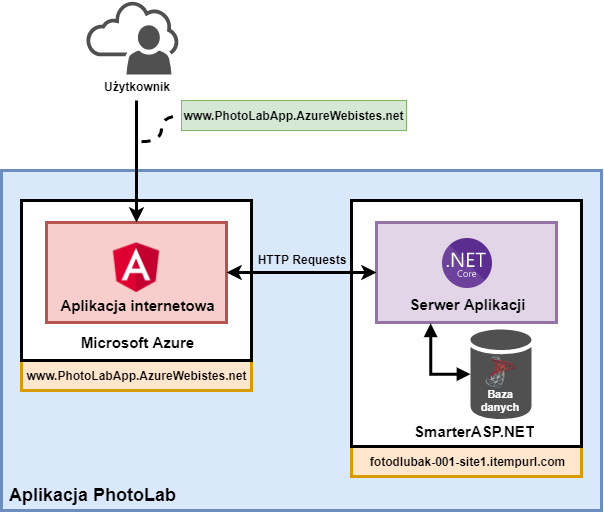
\includegraphics[width=0.8\linewidth]{graphics/chapter-4/production-server.png}
	\caption{Środowisko produkcyjne aplikacji}
	\label{fig:production-server}
\end{figure}

\subsubsection{Wdrożenie aplikacji klienckiej}
\quad Aplikacja kliencka została opublikowana na serwerze znajdującym się w usługach chmurowych oferowanych przez firmę \textit{Microsoft} - \textbf{\textit{Azure}}. Powodem wyboru tego konkretnego usługodawcy jest przede wszystkim zerowy koszt utrzymania. \textit{Azure} w darmowym planie oferowanym przez studencki program partnerski \textit{DreamSpark} w zupełności wystarcza swoimi parametrami technicznymi spełnić wymagania aplikacji \textit{Angular}. Dodatkowo jest on bardzo szybki i zapewnia jedną z najwyższych na rynku dostępności serwera (bardzo dobra stabilność).\\
\\
Proces \textit{deploymentu} należy rozpocząć od zbudowania aplikacji w sposób przeznaczony do działania na serwerze produkcyjnym. W czasie implementacji proces budowania polegał na wykonywaniu komendy:

\vspace{2mm}

    \centerline{\texttt{\hl{ npm start }}}

\vspace{2mm}

\noindent W przypadku potrzeby wygenerowania projektu produkcyjnego należy użyć komendy:

\vspace{2mm}

    \centerline{\texttt{\hl{ ng build --prod }}}

\vspace{2mm}
\noindent W pierwszej jednak kolejności należy założyć konto hostingowe dla serwera (opis w kolejnej sekcji) i w pliku \textit{config.service.ts} podmienić adres \textit{apiURI} na adres WWW serwera wraz z dopisanym na końcu ścieżki - \textit{/api}. Po tym kroku można wykonać powyższą komendę.
Projekt zostanie odpowiednio utworzony w wyznaczonym przez plik \textit{angular-cli.json} miejscu. Dla \textit{PhotoLab} jest to:

\vspace{2mm}

    \centerline{\texttt{\hl{ /Server/wwwroot/ }}}

\vspace{2mm}

\noindent Kolejnym krokiem jest dodaniem do korzenia tak utworzonego projektu (po zbudowaniu projektu, korzeniem staje się folder \textit{/Server/wwwroot}) pliku \textit{web.config} odpowiedzialnego za konfigurację serwera \textit{IIS} odpowiedzialnego za uruchomienie i odpowiednie mapowanie aplikacji na hostingu \textit{Azure}. Kod źródłowy  pliku został zaczerpnięty ze źródła \cite{deploying-angular}.
\newpage

\begin{listing}[ht]
    \xmlcode{listings/web-config.xml}
    \caption{Zawartość pliku \textit{web.config} koniecznego do wdrożenia aplikacji klienckiej}
    \label{listing:web-config}
\end{listing}

        \begin{wrapfigure}[18]{l}{0.4\textwidth}
        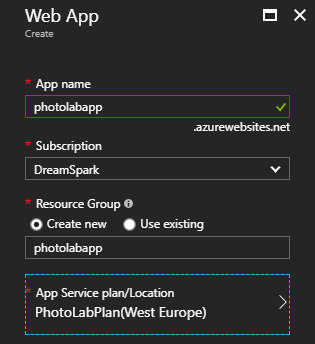
\includegraphics[width=1\linewidth]{graphics/chapter-4/azure-deploy.png}
        \caption{Tworzenie nowej aplikacji Azure}
        \label{fig:azure-deploy}
        \end{wrapfigure}
\noindent Gdy plik zostanie dodany, należy przejść do drugiego etapu wdrożenia. Założenia nowej aplikacji w~portalu \textit{Azure}. W tym celu należy zalogować się na swoje konto do portalu \texttt{https://portal.azure.com}, następnie przejść do zakładki \textit{App Services}, kliknąć przycisk \textit{Add} i~wybrać aplikację typu \textit{Web App}. Kolejnym krokiem jest podanie wymaganych parametrów (Rys. \ref{fig:azure-deploy}). Aplikacja zostanie utworzona. W~zakładce \textit{Deployment credentials} należy ustawić dane dostępowe do serwera \textit{FTP} zgodnie z~własnymi preferencjami.       
 Gdy takowe zostaną określone, wystarczy wykorzystać je do zalogowania się do serwera \textit{FTP} za pomocą dowolnego klienta \textit{FTP} (np. \textit{Total Commander} i przekopiowanie plików z folder \texttt{wwwroot} do katalogu \texttt{site/wwwroot}. \\
 \\
 Aplikacja została poprawnie wdrożona na serwer - adres serwera \textit{FTP} jak i adres \textit{URL} strony na której hostowana jest aplikacja znajduje się w prawej górnej części zakładki \textit{Overview}.
\newpage

\vspace*{0.01\baselineskip}

\subsubsection{Wdrożenie serwera aplikacji i bazy danych}
\quad Aplikacja biznesowa wraz z bazą danych zostały zainstalowane na serwerze obsługiwanym przez firmę \textit{SmarterASP.NET}. Darmowy, 60 dniowy okres testowy wystarczył, aby stwierdzić, iż serwis ten umożliwia stosunkowo proste wdrożenie aplikacji wraz z dołączoną do niej bazą danych. Dodatkowo pierwszy dostępny pakiet cenowy przedstawia bardzo dobry stosunek oferowanych możliwości do kosztów, gdzie zarówno pierwszy, jak i drugi - spełniają wymagania dotyczące serwera produkcyjnego dla aplikacji \textit{PhotoLab}.
        \begin{wrapfigure}[19]{l}{0.35\textwidth}
        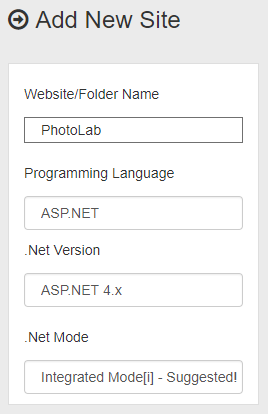
\includegraphics[width=1\linewidth]{graphics/chapter-4/server-account.png}
        \caption{Tworzenie aplikacji smarterASP.NET}
        \label{fig:server-application}
        \end{wrapfigure}
        
\noindent Wdrożenie należy rozpocząć od rejestracji nowego konta w serwisie \textit{SmarterASP.NET}. Następnie należy przejść do panelu zarządzania i z zakładki \textit{Hostings} wybrać przycisk \textit{+~Add New Hosting Account} by utworzyć nowe konto hostingowe. Gdy jest ono gotowe należy z panelu zarządzania hostingiem wybrać \textit{Websites} i zielony przycisk \textit{New Site} w~celu utworzenia struktury nowej aplikacji. Parametry inicjalizacyjne należy ustawić tak jak przedstawiono to na rys. \ref{fig:server-application}.
 Aplikacja zostanie utworzona. Należy pobrać dane wdrożeniowe (\textit{ang. WebDeploy Info}) rozwijając pole \textit{Show WebDeployInfo} i~klikając przycisk \textit{Get Publish Setting} - rysunek \ref{fig:webdeploy-info}.
 
 Kolejnym etapem jest przejście do zakładki \textit{Databases} i~utworzenie bazy danych typu \textit{MSSQL Database}. Gdy baza zostanie stworzona należy postępować podobnie jak w przypadku pobierania \textit{WebDeploy Info}. Rozwinąć zakładkę \textit{Connection String Examples} i zapisać \textit{Connection String} przeznaczony dla aplikacji \textit{ASP.NET}.
 
 \vspace{15mm}
 
\begin{figure}[ht]
	\centering
	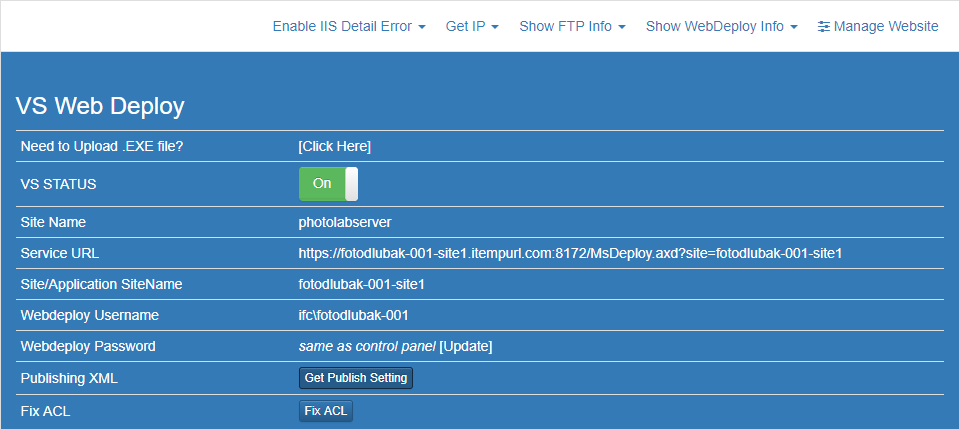
\includegraphics[width=1\linewidth]{graphics/chapter-4/server-webdeploy-info.png}
	\caption{Profil danych koniecznych do wdrożenia serwera}
	\label{fig:webdeploy-info}
\end{figure}

\noindent Ostatnie prace wymagają otwarcia projektu serwera aplikacji w~środowisku \textit{Visual Studio}. Tam w pliku \textit{AppSettings.json} należy podmienić lokalny \textit{Connection String} na ten skopiowany z~utworzonej bazy danych i na jego końcu wprowadzić ustalone do bazy danych hasło. Następnie należy kliknąć \textit{PPM} na nazwę projektu w oknie solucji (\textit{ang. Solution Explorer}) i wybrać publikuj (\textit{ang. publish}).\\
\\
\noindent Kolejne kroki, które należy wykonać to:
 \begin{enumerate}
     \item \textit{Create new profile} -> \textit{import profile} -> \textit{ok}.
     \item Z okna systemowego - wybór pobranego wcześniej profilu.
     \item Z prawej strony rubryki \textit{Summary} wybór: \textit{Settings}.
     \item Wprowadzenie hasła do aplikacji i zweryfikowanie połączenia - \textit{Validate Connection}.
     \item W zakładce \textit{Settings}, ustawienie parametrów jak na rys \ref{fig:server-visual-deploy}, gdzie w polu \textit{ConnectionString} podany jest wcześniej skopiowany link ze zmienionym na końcu hasłem.
     \item Wybranie \textit{Save}, a następnie \textit{Publish}.
 \end{enumerate}
 
 
   \begin{figure}[ht]
	\centering
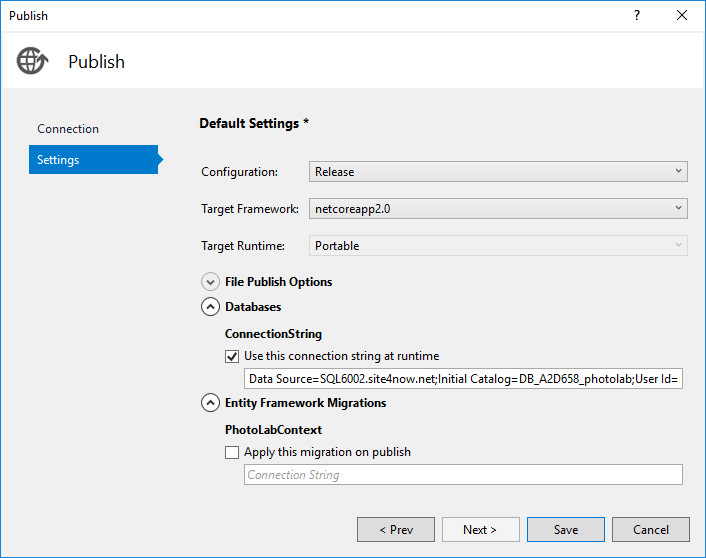
\includegraphics[width=0.7\linewidth]{graphics/chapter-4/server-visual-deploy.png}
\caption{Ustawienia profilu wdrożenia w Visual Studio}
\label{fig:server-visual-deploy}
\end{figure}     
\noindent Po chwili oczekiwania, aplikacja zostanie poprawnie zainstalowana.
Ostatnim wymaganym krokiem jest wykonanie kopii bazy danych (np. poprzez aplikację \textit{Microsoft SQL Server Management Studio}, a następnie jej wgranie na serwer w menu \textit{Databases}, wybierając \textit{Actions}, \textit{Restore Database} i zaznaczając plik kopii bazy danych. Na tym etapie proces wdrożenia dobiegnie końca - strona dostępna jest pod adresem \textit{http://photolabapp.azurewebsites.net}.
\newpage

\vspace*{0.01\baselineskip}

\subsection{Przewodnik użytkownika}
\quad Z racji rozbudowanego interfejsu użytkownika, który zawiera około 30 różnych widoków aplikacji, instrukcja zostanie oparta jedynie o najważniejsze elementy całego serwisu, które są przedstawicielami kategorii poszczególnych stron. Uwzględniony został również podział prezentowanych treści na dwa moduły, które zasadniczo się od siebie różnią - wyglądem, dostępem dla użytkowników i funkcjonalnościami.

\begin{figure}[ht]
	\centering
	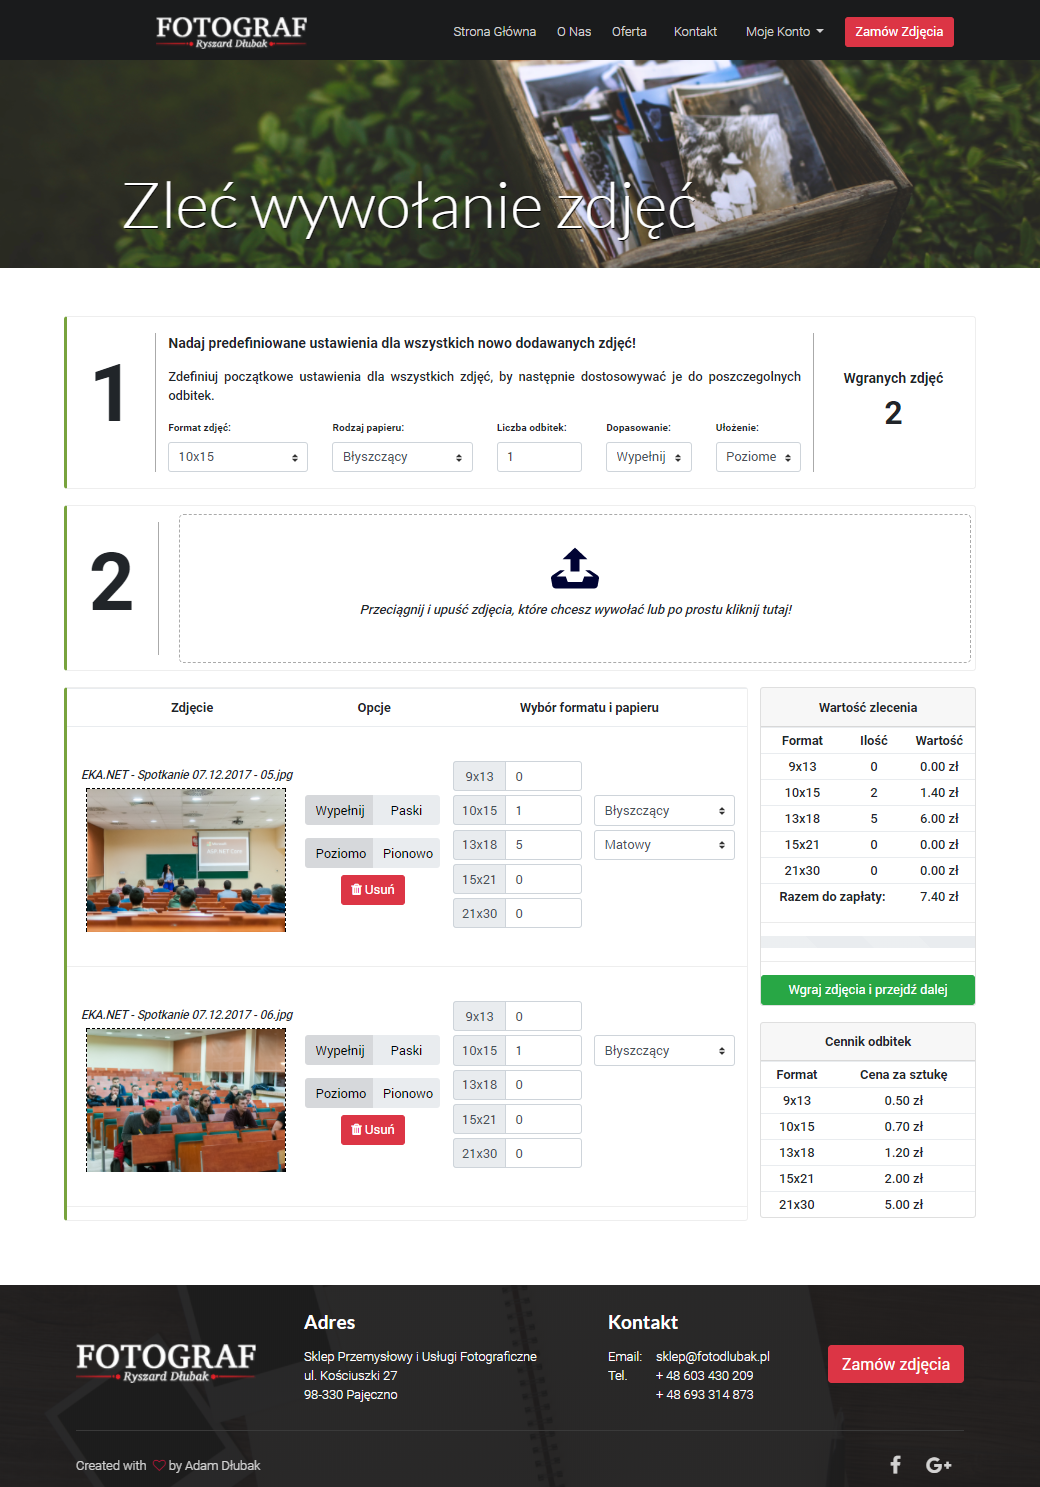
\includegraphics[width=0.85\linewidth]{graphics/chapter-4/screen-1.png}
	\caption{Ogólny widok modułu laboratorium wraz z funkcją zamawiania odbitek}
	\label{fig:screen-1}
\end{figure}
\newpage

\vspace*{0.01\baselineskip}



\subsubsection{Moduł Laboratorium}
\quad Najważniejszym widokiem tego modułu jest oczywiście część odpowiedzialna za \textbf{zlecanie zamówienia} na wykonanie usługi. Pierwszy etap tego procesu wraz z całym kontekstem strony (nagłówek, stopka) został przedstawiony na rysunku \ref{fig:screen-1}. Doskonale widać tam 4 etapy wyboru i parametryzacji zdjęć:
\begin{itemize}
    \item etap 1 - wybór domyślnych parametrów dla wszystkich nowo dodawanych zdjęć,
    \item etap 2 - wgrywanie zdjęć; dwie możliwości - wybór z okna systemowego po kliknięciu w~dostępne pole lub wykorzystanie funkcjonalności ,,przeciągnij i upuść'',
    \item etap 3 - dokładne ustalenie ilości i rodzaju odbitek dla poszczególnych fotografii,
    \item etap 4 - podsumowanie zlecenia i przesłanie plików oraz przejście do kolejnego etapu zamówienia - danych wysyłki, potwierdzenia zakupy i sposobu płatności.
\end{itemize}

\noindent Innym bardzo ważnym zadaniem systemu jest identyfikacja klientów laboratorium. Aby mieć możliwość zlecenia zamówienia, użytkownik zobligowany jest do założenia konta w serwisie, a~następnie za jego pomocą zalogowania się do systemu. \\
\\
Widok \textbf{logowania użytkownika} został przedstawiony na kolejnym rysunku (rys. \ref{fig:screen-2}). Zarówno logowanie jak i rejestracja zostały zaimplementowane w postaci pojawiających się okien - \textit{modali}. Umożliwia to sprawne i wygodne dokonanie autentykacji użytkownika bez opuszczania kontekstu strony, w której się znajdował.

\begin{figure}[ht]
	\centering
	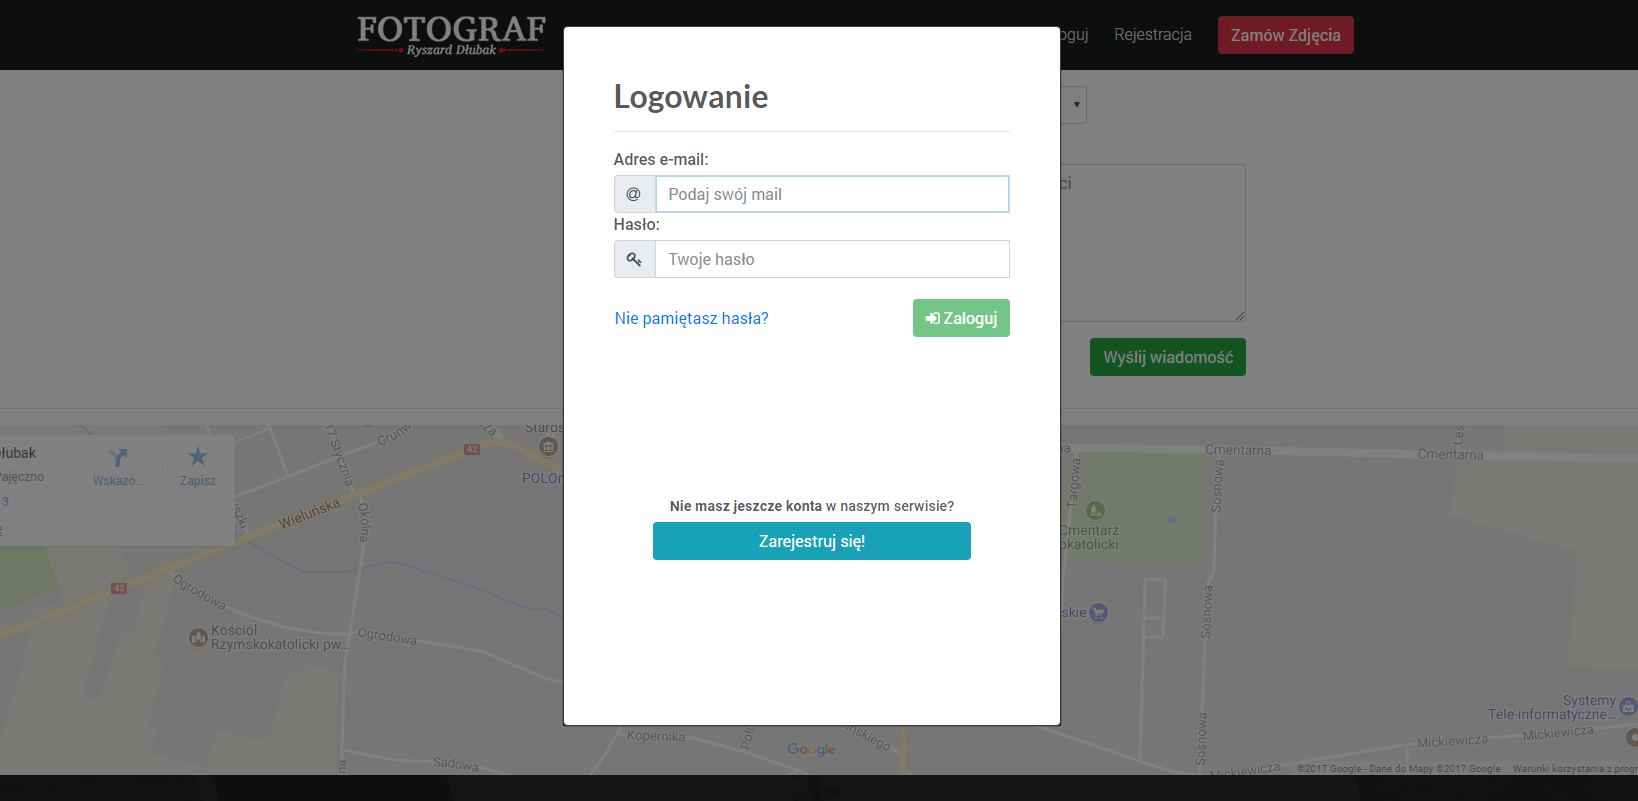
\includegraphics[width=0.9\linewidth]{graphics/chapter-4/screen-2.png}
	\caption{Widok logowania użytkownika}
	\label{fig:screen-2}
\end{figure}

\noindent Klient po zalogowaniu, korzystając z odpowiedniego odnośnika znajdującego się w nagłówku strony (\textit{ang. header}) może przejść do \textbf{panelu użytkownika}. Tam ma możliwość dostosowywania takich parametrów swojego konta jak: podstawowe dane (imię, nazwisko, numer telefonu, adres e-mail), dane do wysyłki zamówienia, dane do faktury, czy zmiana obecnego hasła do konta. Ponadto ma on możliwość przeglądania swoich, zarówno obecnych, jak i już zrealizowanych zleceń.

\begin{figure}[ht]
	\centering
	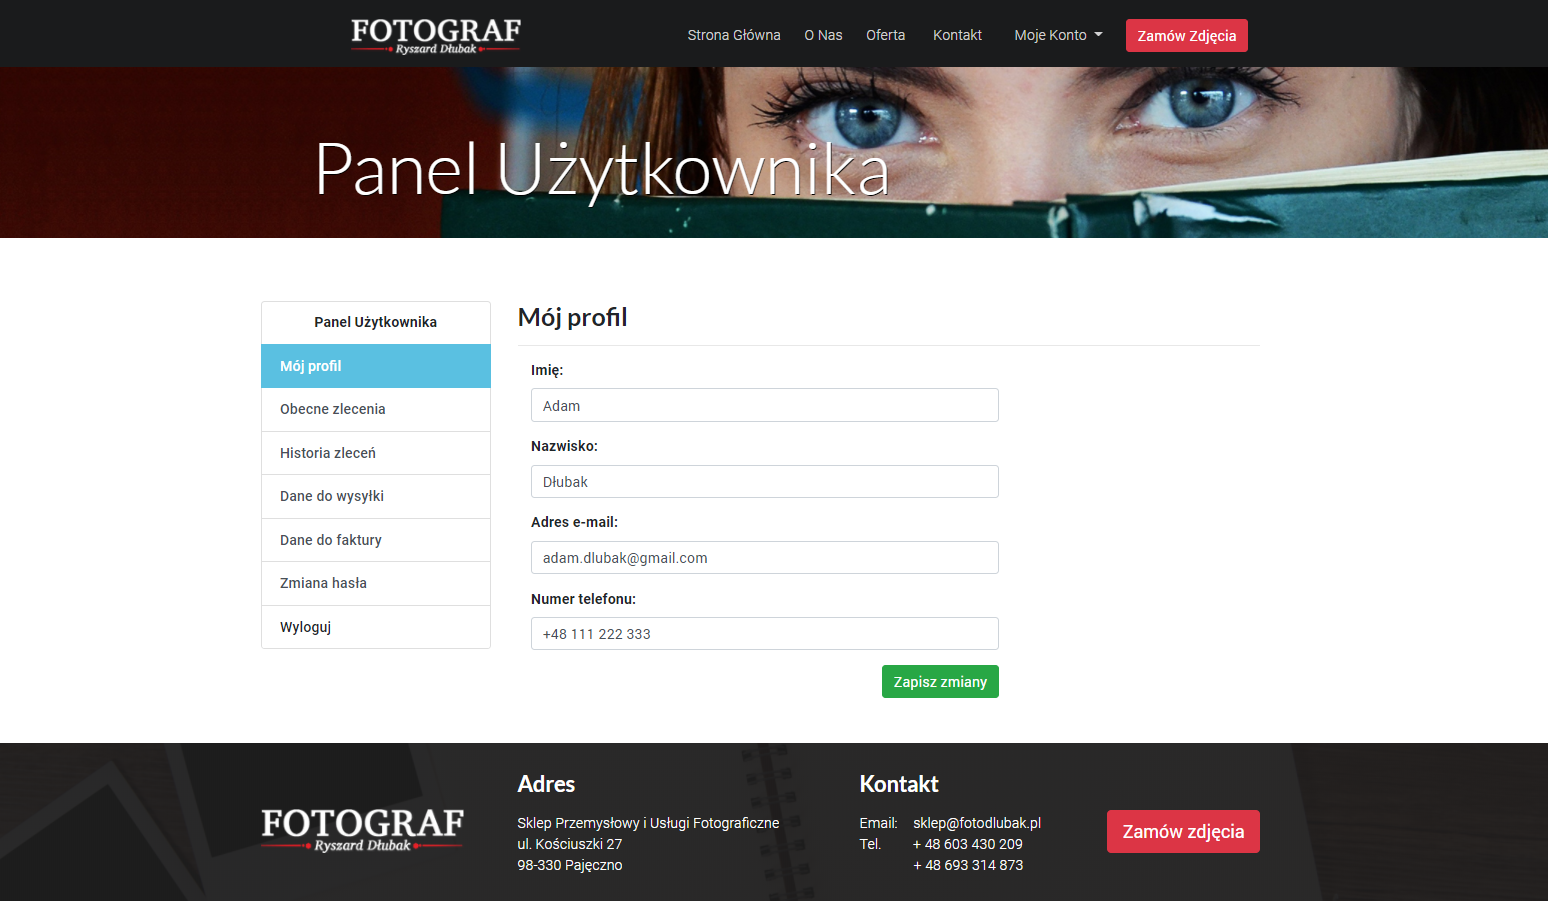
\includegraphics[width=0.85\linewidth]{graphics/chapter-4/screen-3.png}
	\caption{Widok panelu użytkownika}
	\label{fig:screen-3}
\end{figure}

\noindent Oczywiście serwis dostępny dla klienta to nie tylko widoki odpowiedzialne za generowanie zamówień, czy obsługę konta. To również strony prezentujące informacje o firmie, tzw. wizytówki. Wszystkie z tych stron zostały stworzone jako \textbf{strony statyczne}, tj. takie, które nie zawierają treści dynamicznych (np. pobieranych z bazy danych). Jedną z takich stron jest z pewnością podstrona \textit{Kontakt} prezentująca podstawowe informacje o firmie, jej adres, pełną nazwę i dane kontaktowe, a także mapę z zaznaczoną lokalizacją. Ponadto udostępnia ona formularz pozwalający bezpośrednio z poziomu strony internetowej wysłać wiadomość e-mail do laboratorium.

\begin{figure}[ht]
	\centering
	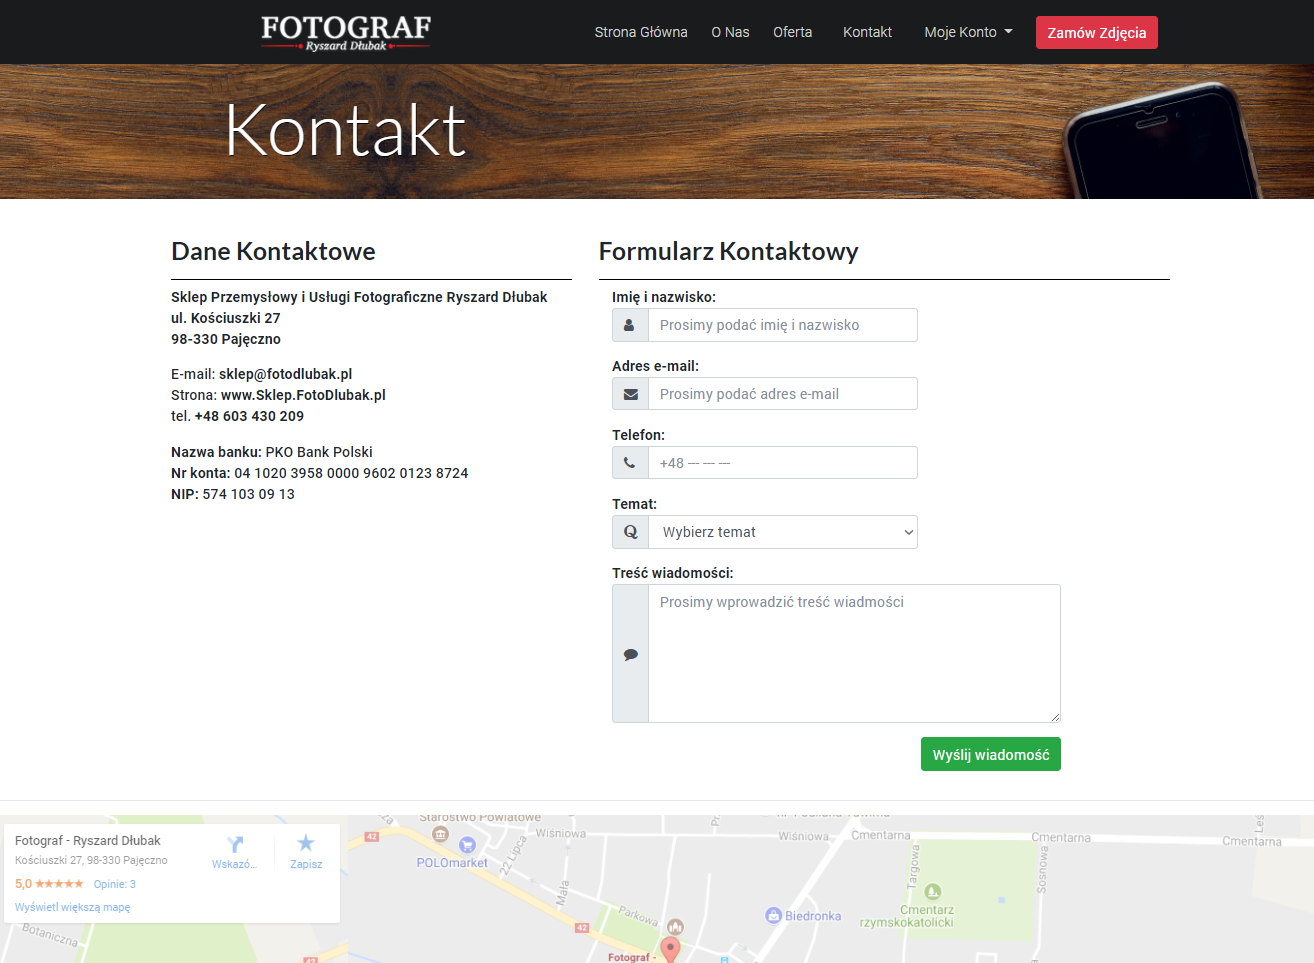
\includegraphics[width=0.85\linewidth]{graphics/chapter-4/screen-4.png}
	\caption{Widok statycznej strony kontaktu}
	\label{fig:screen-4}
\end{figure}

\newpage




\newpage

\vspace*{0.01\baselineskip}


\subsubsection{Moduł Administratora}
\quad Ta część serwisu dostępna jest jedynie dla użytkowników posiadających przedzieloną rolę administratora. Ze względu na swój charakter i prezentowane treści jej \textit{layout} różni się od tego, który udostępniany jest pozostałym użytkownikom aplikacji. Jego zasadnicza część znajduję się po lewej stronie w postaci \textit{sidebara}. Można tam wyróżnić dwa elementy: logo serwisu oraz menu, które umożliwia nawigację do poszczególnych funkcjonalności panelu.\\
\\
Rdzeniem całego modułu jest sekcja dotycząca zamówień. Poprzez wybranie przycisku \textit{Zamówienia}, administratorowi udostępniana jest lista wszystkich zamówień znajdujących się w~systemie. Lista udostępnia takie informacje o zamówieniu jak: data zlecenia, zleceniodawca, ilość odbitek i wartość całego zamówienia, a także jego status. Dodatkowo możliwa jest nawigacja do szczegółów danego zamówienia. Widok ten został zaprezentowany na rysunku \ref{fig:screen-5}.


\begin{figure}[ht]
	\centering
	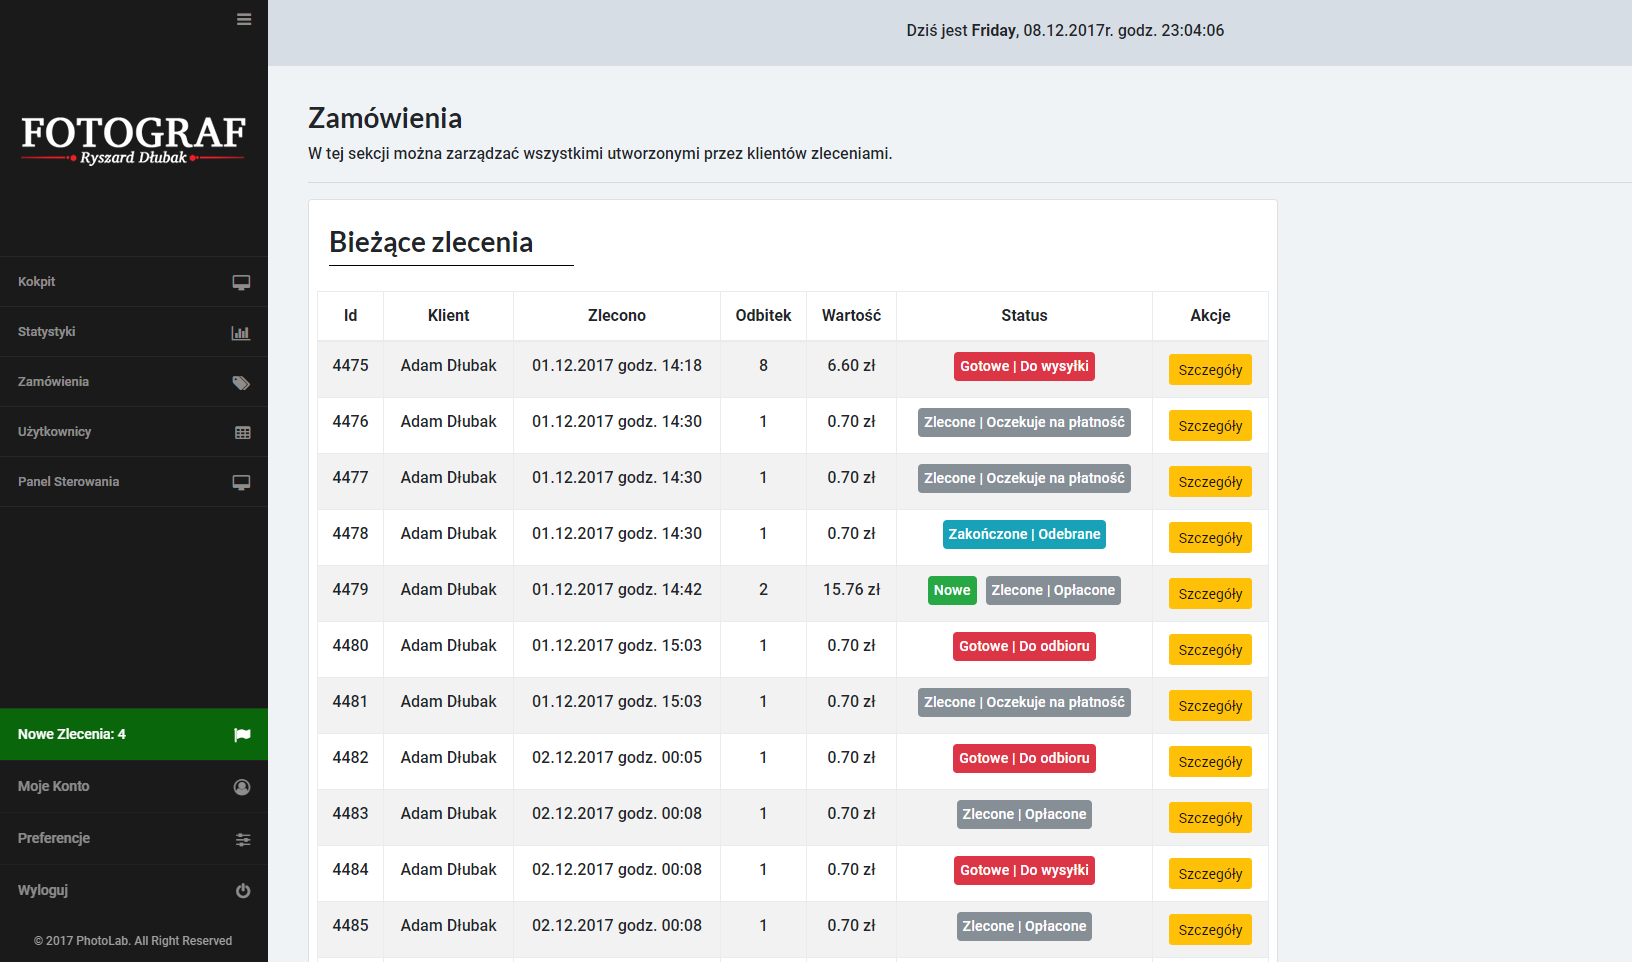
\includegraphics[width=0.9\linewidth]{graphics/chapter-4/screen-5.png}
	\caption{Widok listy zleceń w panelu administratora}
	\label{fig:screen-5}
\end{figure}

\noindent Aby zrealizować zlecenie według wskazań klienta, pracownik zakładu powinien skorzystać z~podglądu całej konfiguracji zlecenia. Udostępnia to kolejny widok zaprezentowany na rysunku \ref{fig:screen-6}.


\begin{figure}[ht]
	\centering
	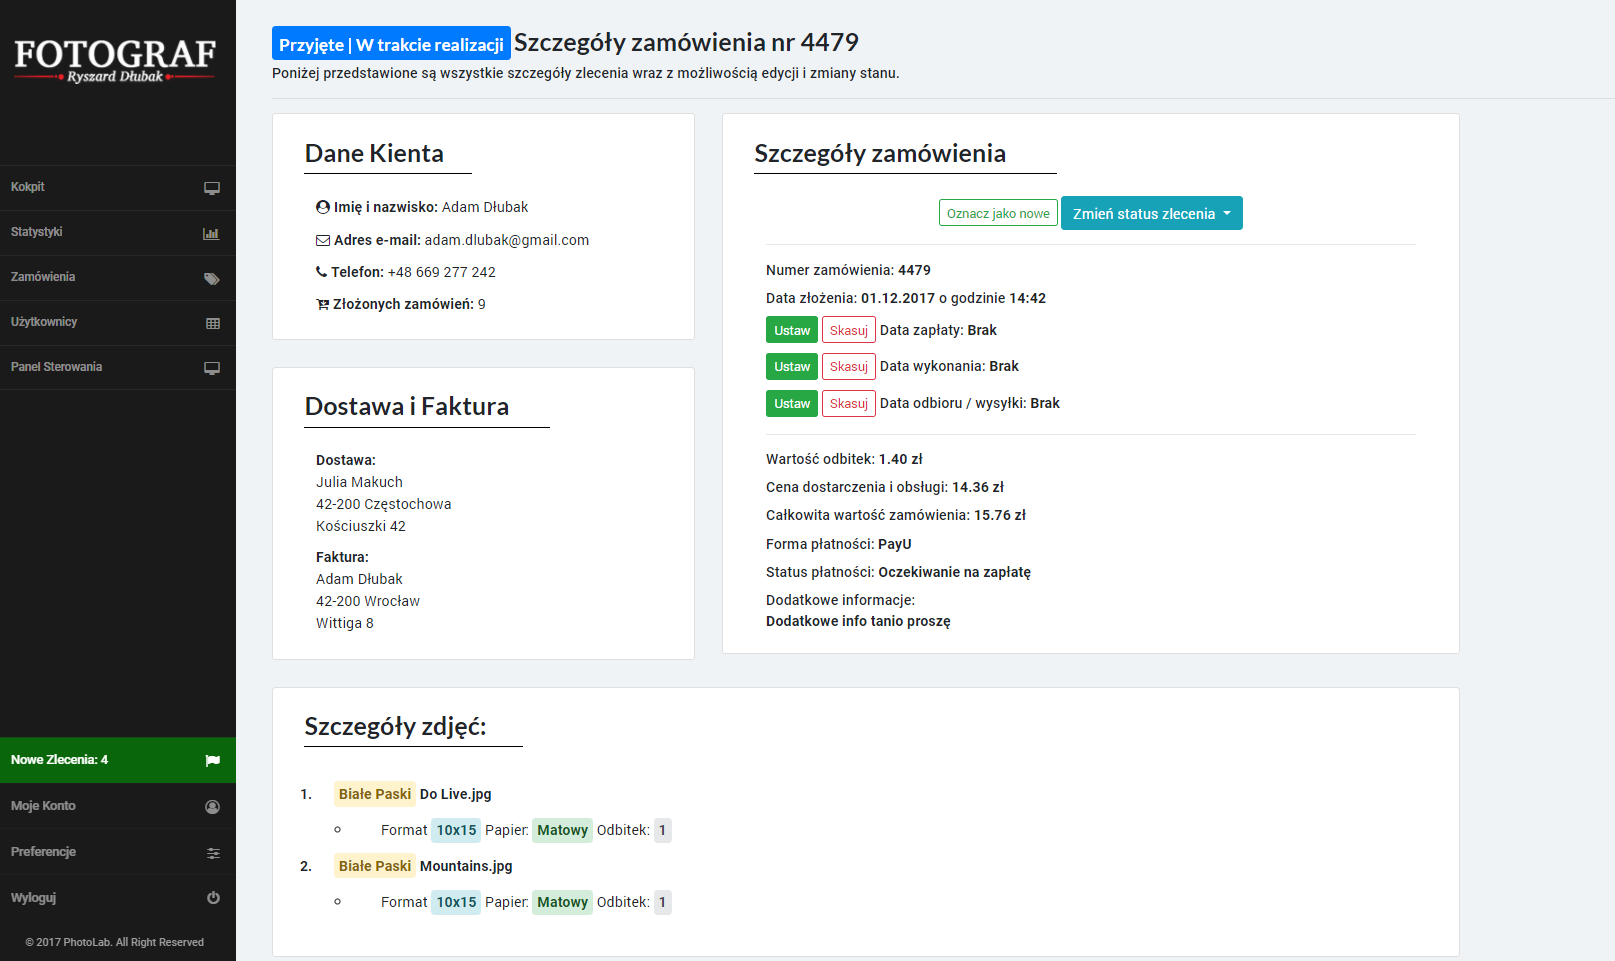
\includegraphics[width=0.9\linewidth]{graphics/chapter-4/screen-6.png}
	\caption{Widok szczegółów zamówienia w panelu administratora}
	\label{fig:screen-6}
\end{figure}

\noindent Ta podstrona ukazuje wszystkie dostępne informacje o zleceniu: podstawowe dane klienta, który je zlecił, a także informacje o adresie wysyłki i wystawieniu faktury. Z prawej strony, w sekcji \textit{szczegóły zamówienia}, administrator ma możliwość dokonania zmiany statusu zlecenia oraz uzupełnienia go o podanie daty jego przejścia do kolejnego etapu realizacji. Trzecią sekcją tego widoku jest część przeznaczona na szczegółowe rozpisanie wymagań dotyczących poszczególnych odbitek. To właśnie według tych treści, pracownik laboratorium realizuje zlecenie wydruku.

\noindent Ostatnim zademonstrowanym widokiem jest podstrona \textbf{panel sterowania}. Dzięki niej możliwa jest konfiguracja ogólnych ustawień serwisu takich jak: dostępne formaty wraz ze szczegółowym ich opisem, rodzaje papieru, czy domyślne ustawienia parametrów podczas dokonywania nowego zlecenia przez użytkowników. Interfejs zapewnia możliwość dodawania, usuwania (lub archiwizacji), a także pełnej edycji wszystkich przedstawionych poniżej ustawień.

\begin{figure}[ht]
	\centering
	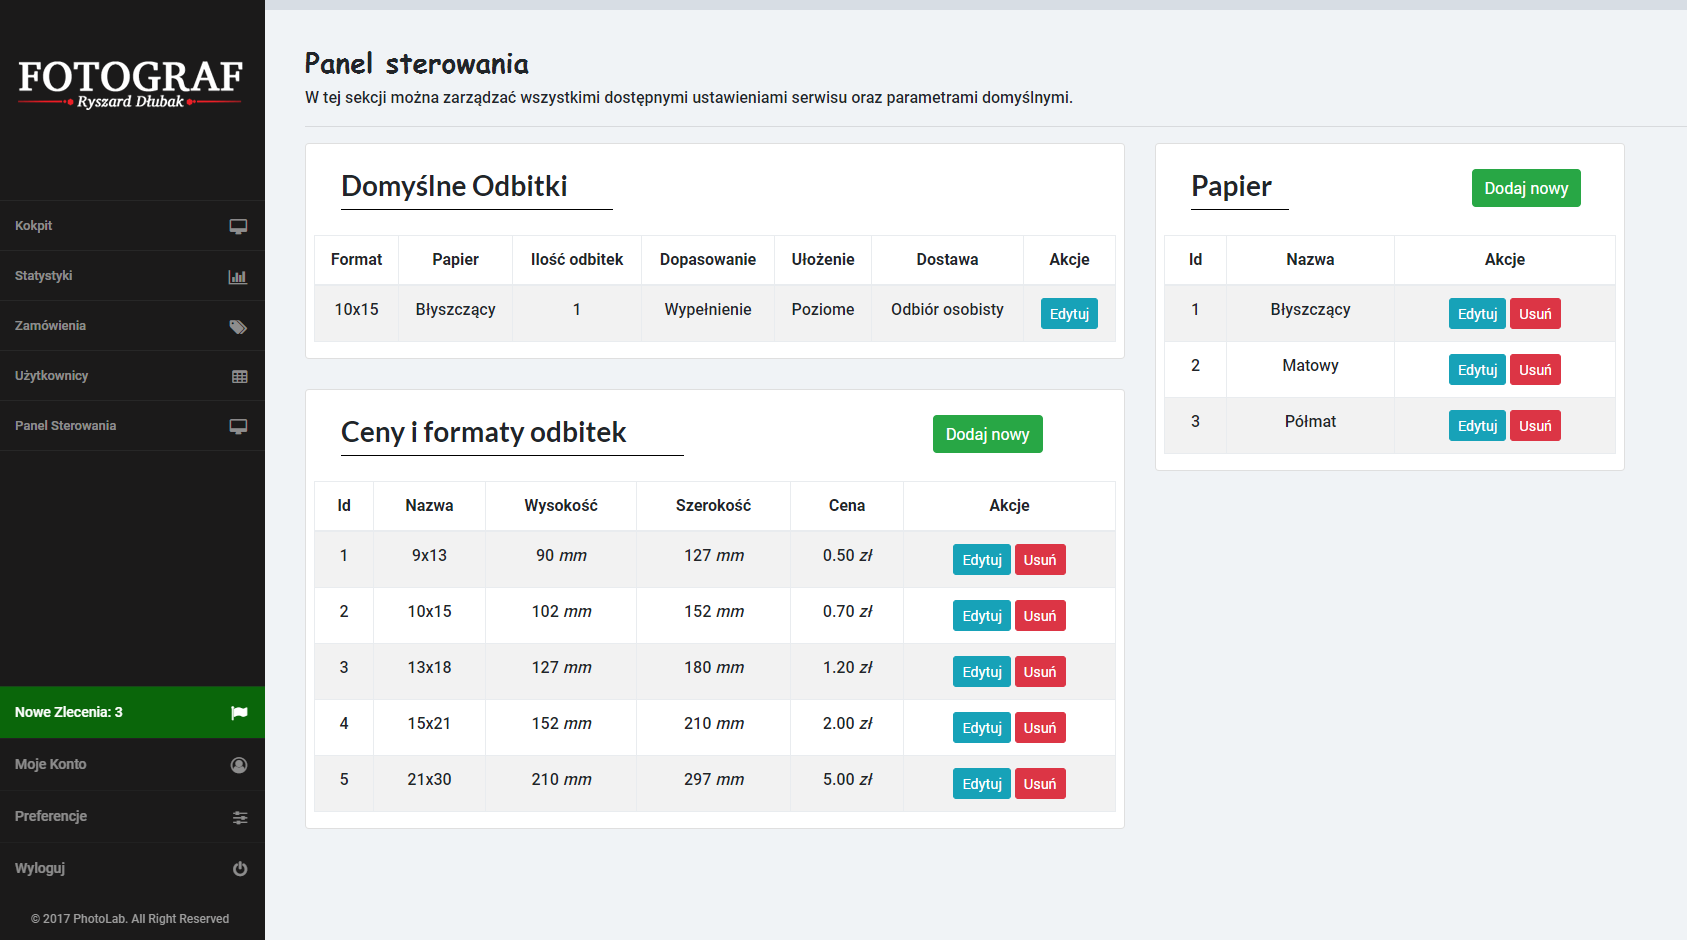
\includegraphics[width=0.9\linewidth]{graphics/chapter-4/screen-7.png}
	\caption{Widok modułu panelu sterowania ustawieniami serwisu}
	\label{fig:screen-7}
\end{figure}

\noindent Moduł administratora to również sekcja zarządzania własnym kontem, a także kontami użytkowników oraz panel statystyk. Nie są to jednak jego najważniejsza opcje, dlatego też zostaną ona pominięte, szczególnie, iż obsługa tej części jest bardzo prosta analogiczna do obsługi zleceń, jak i całego systemu.